\documentclass[a4paper, 11pt]{report}
\usepackage[utf8]{inputenc}
\usepackage{textcomp}
\usepackage[francais]{}
\usepackage{setspace}
\usepackage{graphicx}
\usepackage{tabu}
\usepackage{geometry}
\usepackage{acronym}
\usepackage{minitoc}
\usepackage{amsmath}
\usepackage{mathtools}
\usepackage{algorithm}
\usepackage[noend]{algpseudocode}
\usepackage[sorting=none]{biblatex}
\addbibresource{reference.bib}
\usepackage[T1]{fontenc}
\usepackage{amssymb}
\usepackage{listings}
\usepackage{dirtytalk}
\usepackage{enumitem}
\setlist[enumerate]{itemsep=0mm}
\setlist[itemize]{itemsep=0mm}
\usepackage{graphicx}
\graphicspath{ {./figures/} }


%multiple columns can be created 
\usepackage{multicol}

\usepackage{xcolor}
\usepackage{subcaption}
\definecolor{codegreen}{rgb}{0,0.6,0}
\definecolor{codegray}{rgb}{0.5,0.5,0.5}
\definecolor{codepurple}{rgb}{0.58,0,0.82}
\definecolor{backcolour}{rgb}{0.95,0.95,0.92}

\lstdefinestyle{mystyle}{
	backgroundcolor=\color{backcolour},   
	commentstyle=\color{codegreen},
	keywordstyle=\color{magenta},
	numberstyle=\tiny\color{codegray},
	stringstyle=\color{codepurple},
	basicstyle=\ttfamily\footnotesize,
	breakatwhitespace=false,         
	breaklines=true,                 
	captionpos=b,                    
	keepspaces=true,                 
	numbers=left,                    
	numbersep=5pt,                  
	showspaces=false,                
	showstringspaces=false,
	showtabs=false,                  
	tabsize=2
}

\lstset{style=mystyle}


\usepackage{sectsty}
\chapterfont{\centering}
\geometry{a4paper, tmargin=1in, rmargin=1in, bmargin=1in, lmargin=1in}


\usepackage{cryptocode}



% sets roll number , name and title
\newcommand{\rollno}{roll number}
\newcommand{\name}{name}
\newcommand{\topic}{Title}
\newcommand{\guide}{guide name}
\newcommand{\hod}{HOD name}

\usepackage{fancyhdr}

\pagestyle{fancy}
\fancyhf{}
\renewcommand{\headrulewidth}{2pt}
\fancyhead[R]{\footnotesize{\leftmark}}
%%\fancyfoot[RE,LO]{}
\fancyfoot[C]{\textbf{\thepage}}





\renewcommand*\contentsname{\hfill\textbf{\textbf{\fontsize{16pt}{24pt}\selectfont Table des matières}} \hfill}
\renewcommand{\bibname}{REFERENCES}
\setcounter{tocdepth}{5}
\setcounter{secnumdepth}{5}

%\makeglossaries
\begin{document}
\adjustmtc
\include{mytitle}

\pagenumbering{gobble}
\chapter*{}
\section*{\centering Résumé}


\hspace{4mm} Notre projet de fin d'études consiste à développer une plateforme web destinée aux entreprises pour gérer leurs équipes ainsi que leurs projets. À travers notre solution les utilisateurs peuvent travailler, selon leurs besoins indépendamment l’un de l’autre tout en assurant l’alignement des équipes et des tâches en toute autonomie.
\par Cette plateforme permet d’optimiser le travail en équipe en toute transparence, engagement et responsabilité.


\textbf{\textit{Mots-clés : }}    Spring Boot, Angular, TypeScript, html, PostgreSQL.

\section*{\centering Abstract}
\hspace{4mm}Our end of studies project consists in developing a web platform intended for companies to manage their teams as well as their projects. Through our solution, users can work in their own way, according to their needs, while ensuring the alignment of the teams and tasks with great autonomy.
\par This platform creates a work environment of transparency, commitment and responsibility, to optimize teamworks.

\textbf{\textit{Keywords:}} Spring Boot, Angular, TypeScript, html, PostgreSQL.


\chapter*{\textit{Remerciement}}


\vspace{0.3cm}

\fontsize{12pt}{24pt}\selectfont 
\hspace{4mm}Au terme de ce travail, je voudrais remercier à ceux qui, de loin ou de près, ont apporté leurs encouragements. J'exprime ma gratitude à mes enseignants qui m'ont suivi tout au long de mes études au sein de l’Institut Supérieur des Sciences Appliquées et de Technologie de Sousse.
\par Je tiens à remercier également Mr Mohamed KHALLOULI, directeur général de la société Mocalo Services, de m’avoir accueilli durant six mois afin de réaliser ce stage et de m’avoir permis de travailler avec des outils jusqu’alors inconnus pour moi.
\par Je remercie également mon maître de stage Mr. Ahmed MOUELHI pour sa disponibilité à mon égard, ses judicieux conseils, sa qualité d’écoute et pour son encadrement tout au long du stage.
\par Enfin, mes vifs remerciements s’adressent à Mme Souhaila FKI, maître assistante à l’ISSAT de Sousse, pour ses encouragements et ses précieux conseils durant ce projet. 

%\addcontentsline{toc}{chapter}{Dédicaces}
\pagenumbering{roman}
\chapter*{}
\section*{\centering \textit{Dédicaces}}
\begin{center}
\vspace{6mm}
\textit{De tout mon cœur, avec mes sincères \\sentiments de reconnaissance et de gratitude, je dédie mon travail\\ à ma famille qui m’a énormément encouragé durant mes études et pour ses sacrifices. \\Pour mes amis qui m’ont donné l’espoir et l'appui dont j’ai besoin.\\ Et pour ceux qui ont participé dans ce projet.\\
J’espère avoir répondu à vos attentes. }



\end{center}
\renewcommand{\listtablename}{Liste des tableaux}
\renewcommand{\listfigurename}{Liste des figures}
%\renewcommand{\Glossairedesacronymes}{Glossaire des acronymes}
\tableofcontents

\cleardoublepage
\addcontentsline{toc}{chapter}{\listfigurename}
\listoffigures

\cleardoublepage
\addcontentsline{toc}{chapter}{\listtablename}
\listoftables

\cleardoublepage
%\printglossaries
\addcontentsline{toc}{chapter}{Glossaire des acronymes}

\chapter*{Glossaire des acronymes }
\markboth{\MakeUppercase{Glossaire des acronymes}}{}

\adjustmtc
\thispagestyle{plain}

   \textbf{HTTP}   \hspace{8mm}  HyperText Transfer Protocol     \\
  \hspace{4mm}  \textbf{UML}   \hspace{10mm}     Unified Modeling Language  \\
\hspace{4mm}  \textbf{CSS}   \hspace{12mm}     Cascading Style Sheets 
  \\
\hspace{4mm}  \textbf{HTML 
}   \hspace{5mm}     HyperText Markup Language  
  \\
\hspace{4mm}  \textbf{SSII 
}   \hspace{11mm}     Société de Services en Ingénierie Informatique 
  \\
\hspace{4mm}  \textbf{STS 
}   \hspace{11mm}     Spring Tool Suite
  \\
\hspace{4mm}  \textbf{IDE }   \hspace{11mm}     Integrated Development Environment
  \\
\hspace{4mm}  \textbf{API }   \hspace{11mm}     
Application Programming Interface
%\acro{}{}
%\acro{}{}




\cleardoublepage
\addcontentsline{toc}{chapter}{Introduction Générale}
\mark{INTRODUCTION GÉNÉRALE}
\pagenumbering{arabic}
\thispagestyle{plain}
\mark{ INNTRODUCTION GÉNÉRALE}
\begin{center}
	\textbf{\textbf{\fontsize{16pt}{24pt}\selectfont Introduction Générale}}
\end{center}
\vspace{0.3cm}
% Enter the title of your project in the section where it says PROJECT NAME
\fontsize{12pt}{24pt}\selectfont
\hspace{4mm}De nos jours les objectifs de chaque entreprise sont d’une part, la satisfaction de ses clients à travers des services répondant à leurs attentes et réalisés dans les budgets et les délais impartis, et d’autre part l’optimisation des ressources afin que l’entreprise puisse réaliser ses travaux de manière rentable.
  
Les années dernières, les entrepreneurs étaient confrontés à un problème majeur celui du développement rapide de leurs entreprises tout en maintenant leurs niveaux d’engagement, de productivité et de satisfaction de leurs collaborateurs. Il manquait une plateforme efficace et transparente pour tout gérer.

C’est dans ce cadre que s’inscrit mon travail de PFE. En effet, il s’agit de développer une application de gestion de projets dédiés aux entreprises de toutes tailles et dans tous les secteurs. Cette plateforme relie les membres qui appartiennent à une telle entreprise, et renforce l’efficacité de travail en offrant un Work Operating System (work OS) qui permet la collaboration et la maitrise des actions par les équipes de l’entreprise. Mocalo, l'entreprise où j'ai effectué mon stage se présent aujourd’hui avec la conviction que la transparence et la collaboration créent une culture de responsabilité et d’autonomie. En effet, plus les équipes de travail sont autonomes, plus elles sont productives.
\par A travers ce rapport je vais présenter mon projet ainsi que la démarche qui a aboutie à la réalisation de ce dernier. Le premier chapitre décrit le cadre du projet. Le deuxième chapitre est consacré à la phase d’analyse et de spécification des besoins. Le troisième chapitre détaille la conception de notre plateforme ainsi que l’environnement de travail. Enfin, le dernier chapitre résume les différentes phases de réalisation de cette plateforme. 




\chapter{ Cadre du projet} \label{ch:Organisme_d'accueil}


\hspace{4mm}
Dans ce chapitre, nous commençons par une présentation de l'entreprise d'accueil "Mocalo". par la suite nous décrivons la problématique puis nous introduisons le cahier des charges de projet. Enfin, nous détaillons notre plan de travail.

\section{ Présentation de l’entreprise }

\hspace{4mm} MOCALO SERVICES est une société créée le 03 Octobre 2019, suite à un constat d’un fort besoin de conseils pour les entreprises de différents domaines. Elle est spécialisée dans le secteur d'activité de conseil en systèmes et logiciels informatiques.
\begin{figure}[h]
    \centering
    
\includegraphics[scale=0.2]{figures/aniskab.jpg}
    \caption{Logo Mocalo}
    \label{fig:logo_mocalo}
\end{figure}
\subsection{ 	Les rapports sociaux : }

\begin{itemize}
    \item	\textbf{Entre ouvriers :} Dans l’ensemble, les rapports sont amicaux et très entretenus. On avait l’habitude de venir 10 à 15 minutes avant l’heure de travail le matin pour avoir l’occasion de boire un café et discuter ensemble. 
\newpage    \item \textbf{Entre chefs et ouvriers :} Le schéma de base où le chef donne les ordres et l’ouvrier les exécute est rarement respecté dans l’entreprise. En effet, les ouvriers maitrisent leurs métiers et remplissent leurs fonctions avec les outils qu’ils ont et les chefs supervisent toutes les opérations et les valident.
\end{itemize}
\subsection{	Organigramme de l’entreprise  :}
\hspace{4mm}L’organigramme de la figure \ref{fig:bureau} montre une représentation schématique des liens hiérarchiques de l'organisme d'accueil. Il sert à donner une vue d’ensemble de la répartition des postes et fonctions au sein de l'entreprise. 
\begin{figure}[h]
		\centering
		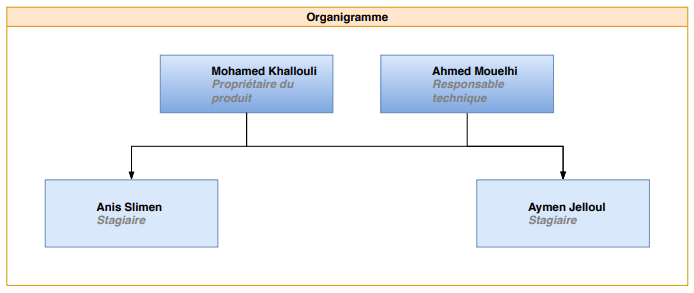
\includegraphics[scale=0.7]{figures/a10.png}
		\caption{Organigramme de l'entreprise}
		\label{fig:bureau}
\end{figure}

 \section{	Présentation du projet  }
 \subsection{	Problématique}
\hspace{4mm} Une des tendances les plus en vue et qui concerne tous les secteurs de développement informatique, est la numérisation. Depuis l’apparition de l’informatique et son introduction dans le monde économique, les entreprises et les entités publiques aspirent à optimiser et à rendre fiable la gestion de leurs structures internes.
\par A l’instar de toute entreprise, une SSII veut améliorer ses procédures de gestion des projets, pour disposer d’une vision globale des différents projets et de leurs états d’avancement.
\par Le succès d’un projet se mesure à la satisfaction du client et à la qualité du résultat, c’est-à-dire à la conformité du produit à ce qui est attendu et à sa livraison dans le respect du délai imparti et du budget alloué.
\par Au cours d’un projet, on est susceptible de confronter plusieurs risques à savoir:
\begin{itemize}
    \item Le risque de dépassement du budget.
    \item Le risque de dépassement des délais.
    \item Le risque d’abandon du projet.
\end{itemize}
\par Sans oublier le risque majeur qui peut toucher la gestion d'un projet et qui est l'absence ou la mauvaise communication entre les différents intervenants. 

\par ainsi pour dépasser tous les risques précédemment cités nous avons proposé une solution informatique à la fois simple, pratique et robuste.


\subsection{	Objectifs}
  \hspace{4mm}  Dans le cadre de mon projet de fin d’études en Génie logiciel, à l’Institut Supérieur des Sciences Appliquées et de Technologie de Sousse, je suis chargé de développer une application qui va servir de menu permettant d’effectuer des tâches spécifiques selon le profil de l’utilisateur.  
\par Chaque tâche devra répondre aux besoins de l’organisme comme par exemple établir un suivi de projet afin d’avoir une vision globale de l’avancement du projet. Il est aussi recommandé de mettre en place des recherches simples et multicritères pour effectuer des opérations d’ajout, de suppression et de modification sur les informations présentes dans la base de données définie préalablement.
\section{	Étude de l'existant}
\hspace{4mm} Nous ne saurions commencer ce travail et élaborer la solution proposée sans avoir une idée claire et précise sur l’existant. La première tâche dans notre projet était la recherche de ce qui est existant sur le marché numérique. Dans ce qui suit nous présentons quelques exemples d’applications ayant plus ou moins des fonctionnalités similaires à celles de notre projet dans le but de dégager leurs limites, ce qui va nous permettre de mettre en relief notre valeur ajoutée par rapport à ce qui existe déjà.

\begin{figure}[h]
		\centering
		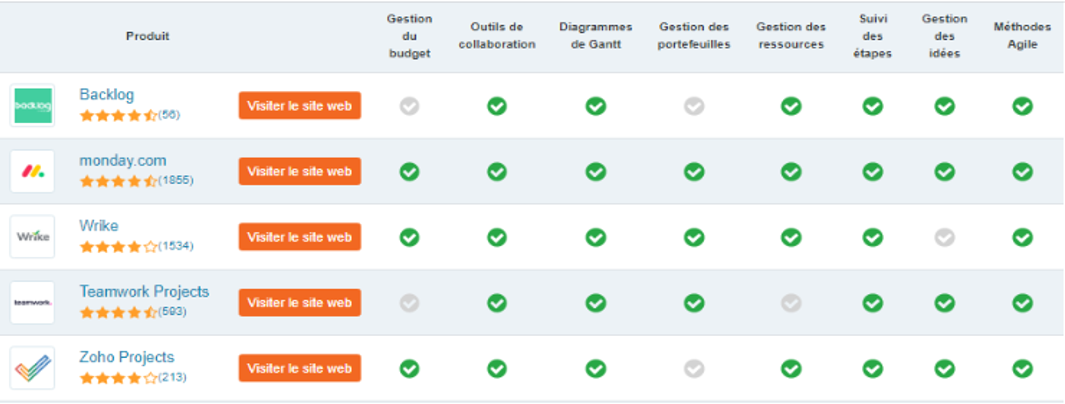
\includegraphics[scale=0.45]{figures/333ANIS3.png}
		\caption{Etude de l’existant}
		\label{fig:etudex}
\end{figure}\par Avant d’entamer une étude détaillée du projet, il nous a fallu réaliser une étude de l’existant sur le marché numérique ce qui nous a montré des insuffisances et plusieurs problèmes qui couvrent plusieurs préoccupations :
\begin{itemize}
    \item préoccupation en termes de rapidité : Comment accélérer le processus de travail au sein d’une entreprise de façon à gagner le maximum de temps ?
    \item préoccupation en termes d’accessibilité : Comment fournir aux utilisateurs un portail numérique simple et facile à exploiter ?
    \item Préoccupation en termes d’efficacité : Comment garantir une solution qui satisfait les besoins de l’utilisateur ?
\end{itemize}
\section{Solution proposée}

\hspace{4mm}    Notre solution consiste à développer une plateforme web de gestion de projets. Cette plateforme permet, d’une manière centralisée, d’aider les sociétés de services à la gestion des tâches, notamment au suivi de projets, du temps et de la collaboration en équipes. 

\section{	Chronologie}
\hspace{4mm}La planification est parmi les phases d'avant-projet. Elle consiste non seulement à délimiter le périmètre temporel du projet, mais aussi à prévoir le déroulement des activités tout au long de la période allouée au stage. La figure suivante détaille la planification temporelle du projet :
% \begin{center}
% \begin{tabular}{|c|l|l|l|l|l|l|l|l|l|l|}
% \hline 
% Produit & Gestion  & Outils de  & Diagramme  & Gestion des  & Gestion des  & suivi des  & Gestion  & Méthodes \\&de budget&collaboration&de Gantt&portfeuilles&ressources&étapes&des idées&Agile
% \\\hline 
%     Backlog &%
\includegraphics{figures/aniska.png}
% & & & & & & &\\\hline 
%     monday.com & & & & & & & & \\\hline
%     Wrike & & & & & & & & \\\hline 
%     Teamwork Projects & & & & & & & & \\\hline 
    
% \end{tabular}
% \captionof{table}{Description du processus de l’authentification}
% \label{desc_auth}
% \end{center}

\begin{figure}[h]
		\centering
		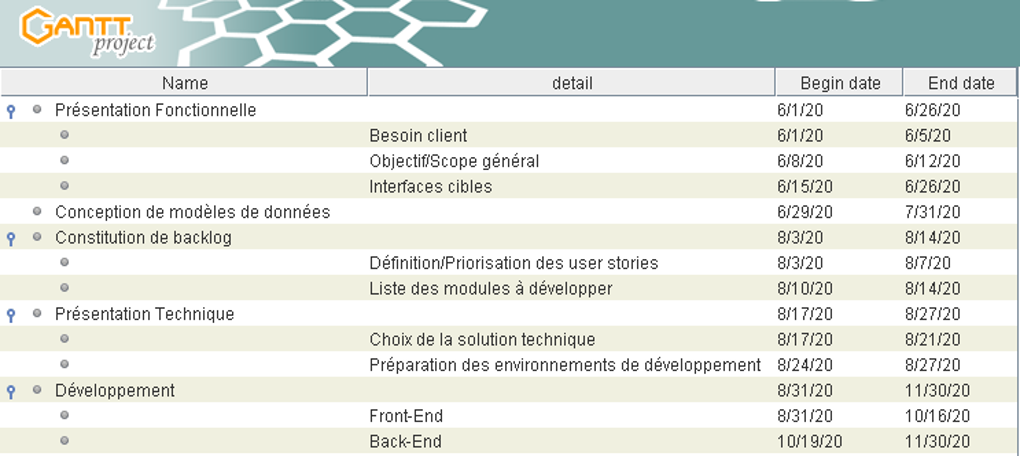
\includegraphics[scale=0.9]{figures/anis3.png}
		\caption{Diagramme de GANTT}
		\label{fig:gantt}
\end{figure}
\section{	Processus de développement}
\hspace{4mm}Agile est un ensemble de méthodes et de processus, orienté collaboratif, transversalité et autonomie ; dont les grands principes sont notamment exposés dans le manifeste Agile.
\par Parmi les méthodologies agiles les plus utilisées est Scrum que nous avons choisie d'utiliser pour notre projet. 
\par La méthodologie scrum, offre plusieurs avantages : Elle assure la livraison de l’application dans les bons délais, tout en fournissant un produit qui respecte les attentes du client. Cela, nous permet d’obtenir une application plus flexible qui s’adapte plus facilement aux nouveaux changements.\newpage



\section*{Conclusion}
\hspace{4mm} Ce chapitre est considéré comme la partie introductive de notre projet, dont laquelle nous avons dégagé la problèmatique , ensuite nous avons récapitulé une idée générale sur les différentes applications existantes ayant plus ou moins des fonctionnalités similaires à celles de notre projet et enfin nous avons présenté notre solution. Le chapitre suivant présentera la spécification des besoins afin d'atteindre les objectifs fixés pour notre projet.

	



\chapter{ Spécification des besoins} \label{ch:specification_techniq}
\hspace{4mm} Dans ce chapitre, nous abordons la phase d’analyse et spécification des besoins. Ainsi, nous présentons les besoins fonctionnels et non fonctionnels de notre système. Nous décrivons ensuite les principaux cas d'utilisation par le language UML qui représente un moyen simple et facile à comprendre.
\section{	Besoins fonctionnels }
\hspace{4mm} Cette partie décrit les exigences que le système doit satisfaire d’une façon informelle. 
\par Les fonctionnalités qu’on propose de fournir dans notre plateforme sont les suivantes:
\par \textbf{Gestion de projet}
\begin{itemize}
    \item	Chaque projet a un responsable qui peut être un chef de projet ou un membre de l’équipe.
    \item 	Le responsable peut réassigner le projet à n’importe quel utilisateur.
    \item Le responsable de projet a toutes les autorisations pour gérer le projet (modification, ajout ou affectation des tâches….).
    \item Un projet peut avoir plusieurs personnes qui travaillent dessus.
    \item Le chef de projet peut avoir plusieurs projets. 
    \item 	Tous les membres de l’entreprise peuvent voir les états des projets grâce aux diagrammes de GANTT.
    \item 	L'invité (qui va être introduit ci-dessous) peut consulter des cartes et des diagrammes de GANTT.
    \item L'invité peut recevoir des notifications de réunions.
\end{itemize}
\par \textbf{Gestion des tâches}
\begin{itemize}
    \item 	Chaque tâche a un responsable qui peut être le chef de projet, le chef d'équipe ou un membre de l’équipe.
    \item 	Le responsable d’une tâche a les autorisations de modification sur la tâche.
    \item 	Une tâche fait partie d’un seul projet.
    \item 	Chaque membre d’un projet peut participer à plusieurs tâches.
    \item Chaque membre d’un projet peut commenter une tâche comme il peut commenter le projet.
\end{itemize}
\par\textbf{Emploi du temps}
\begin{itemize}
    \item 	Chaque membre doit entrer toutes ses heures de travail.
    \item 	Chaque heure entrée correspond à une tâche du projet.
    \item L’entrée des heures de travail se fait le jour même où le jour suivant.
    \item La saisie des vacances, maladies et autres congés se fait dans la plateforme.
    \item 	Le chef d'équipe doit valider les emplois du temps.
    \item 	Le chef d'équipe peut saisir les emplois du temps pour les membres de son équipe.
    \item 	Le chef d'équipe peut saisir les prévisions de congés d'un autre membre de son équipe.
\end{itemize}
\par\textbf{Gestion des ressources humaines}
\begin{itemize}
    \item 	L’administrateur peut ajouter, modifier et supprimer des membres d’une équipe de travail.
    \item 	L’administrateur peut ajouter et modifier des équipes de travail.
    \item Le chef de projet peut éditer les autorisations d'un membre d’une équipe.
\end{itemize}
\par \textbf{Gestion de communication}
\begin{itemize}
    \item 	Le membre d’un projet peut organiser des réunions s'il a l’autorisation de le faire.
    \item 	L’invité peut participer à des réunions.
    \item Le membre d’un projet peut envoyer/corriger des comptes rendus suite à une réunion s’il y a participé.
    \item 	Le membre d’un projet peut recevoir des comptes rendus.
\end{itemize}
\section{	Besoins non Fonctionnels}
\hspace{4mm}Ce sont des exigences qui ne concernent pas spécifiquement le comportement de la plateforme mais plutôt qui identifient des contraintes internes et externes de la plateforme. 
\par Les principaux besoins non fonctionnels de notre plateforme se résument dans les points suivants :
\begin{itemize}
    \item \textbf{	Ergonomie : }notre application doit offrir une interface conviviale et ergonomique exploitable par l'utilisateur en envisageant les interactions via le navigateur web.
    \item \textbf{	Compatibilité : }l’un des points les plus importants lors du développement d’une application sur un environnement web ou mobile, c’est d’assurer sa compatibilité avec toutes les versions du système ; n’importe quels version et type de navigateur.
    \item \textbf{	La sécurité de l’accès aux informations critiques : }nous devons prendre en considération la confidentialité des données des utilisateurs à travers Spring security et JWT surtout au niveau de l’authentification.
    \item \textbf{	Maintenabilité : }Pendant la phase de maintenance, le code de notre application doit être facile à lire et à comprendre. À cette fin, nous avons décidé de bien commenter le code pour le rendre facile à comprendre et d’utiliser des noms significatifs pour les classes et les variables.
    \item \textbf{	Les contraintes de disponibilité : }l’application doit être disponible pour être utilisée par n’importe quel utilisateur.
\end{itemize}
\section{	Diagrammes de cas d'utilisation}
\hspace{4mm}Dans ce qui suit, nous présentons un formalisme semi formel de spécification des besoins de notre système, à l’aide de diagrammes de cas d’utilisation accompagnés par une description textuelle.
\par Cette description permet de clarifier le déroulement de la fonctionnalité et d’identifier les parties redondantes pour en déduire des cas d’utilisation plus précis qui seront utilisés par inclusion, extension ou généralisation.
\par Dans sa forme textuelle un cas d’utilisation est une collection de scénarios de succès et d’échecs qui décrivent la façon dont un acteur particulier utilise le système pour atteindre un objectif.
\par Les termes suivants sont utilisés pour chaque cas d’utilisation :
\begin{itemize}
    \item \textbf{ Précondition : }définit ce qui doit être vrai en amont afin que le processus puisse démarrer.
    \item \textbf{	Déclencheur : }action qui déclenche le scénario.
    \item \textbf{ Scénario nominal : }scénario qui satisfait l’objectif des acteurs par le chemin le plus direct.
    \item \textbf{	Extensions : }tous les autres scénarios ou branchements possibles aussi bien de succès que d’échec.
\end{itemize}
\subsection{	Identification des acteurs}
\hspace{4mm}Un acteur représente un rôle joué par une entité externe qui interagit directement avec la plateforme mise en place. Il peut consulter et/ou modifier directement l’état du système, en émettant et/ou recevant des messages susceptibtles d’être porteurs de données. \cite{1}
\par Les acteurs suivants ont été identifiés :
\begin{itemize}
    \item 	Invité : qui a des droits de consultation uniquement.
    \item  Membre de la société : qui a des droits restreints sur le projet en question et qui peuvent être définis par le chef de projet.
    \item Chef de projet : qui a des droits sur les projets et les équipes sous sa responsabilité.
    \item	Chef d’équipe : qui est un membre responsable d’une ou de plusieurs équipes.
    \item 	Administrateur : qui est un membre qui s’occupe de l’administration de l’entreprise.
\end{itemize}
\par Il existe des relations d’héritage entre les différents acteurs :
\begin{itemize}
        \item[-] Les invités sont étendus en des membres.
        \item[-] Les membres sont étendus en chefs de projet.
        \item[-] Les chefs de projets sont étendus en chefs d'équipes.
        \item[-] Les chefs d’équipes sont étendus en administrateur, qui a des privilèges supplémentaires comme on peut le voir sur le diagramme "Diagramme de cas d’utilisation Invité " (figure \ref{fig:cas_invi}).
\end{itemize}
\subsection{ Identification des cas d’utilisation}
\hspace{4mm}Les cas d’utilisation représentent un ensemble de séquences d’actions qui sont réalisées par le système et qui produisent un résultat observable intéressant pour un acteur principal. 
\par Dans la collection des cas d’utilisation, sont énumérés tous les processus principaux du système à savoir :
\begin{itemize}
    \item 	Authentification
    \item 	Réception des comptes rendus
    \item 	Participation à des réunions
    \item	Réception des notifications
    \item	Gestion des tâches
    \item	Faire des recherches
    \item	Géstion des les comptes rendus
    \item	Organisation des réunions
    \item	Modification de ses informations
    \item	Saisie de l'emploi du temps
    \item	Saisie des commentaires
    \item	Saisie des prévisions de congés
    \item	Gestion de projet
    \item	Assignation des tâches
    \item	Edition des autorisations pour un autre membre
    \item	Edition des abonnées
    \item	Suivi de projet
    \item	Validation des emplois du temps
    \item	Saisie des emplois du temps de son équipe
    \item	Saisie des prévisions de congés pour son équipe
    \item	Gestion des utilisateurs
    \item	Souscription d'une offre
    \item	Paramétrage général
    \item	Gestion des équipes
\end{itemize}\newpage
\subsection{	Diagrammes généraux}
\hspace{4mm}Dans cette partie, nous présentons les diagrammes des cas d’utilisation détaills ainsi que leurs descriptions textuelles.
\par	\textbf{L’invité :}c’est une personne qui est invitée par email à la plateforme pour recevoir des notifications concernant un projet, participer à une réunion et recevoir des comptes rendus ou des cartes et des diagrammes.

\begin{figure}[h]
    \centering
    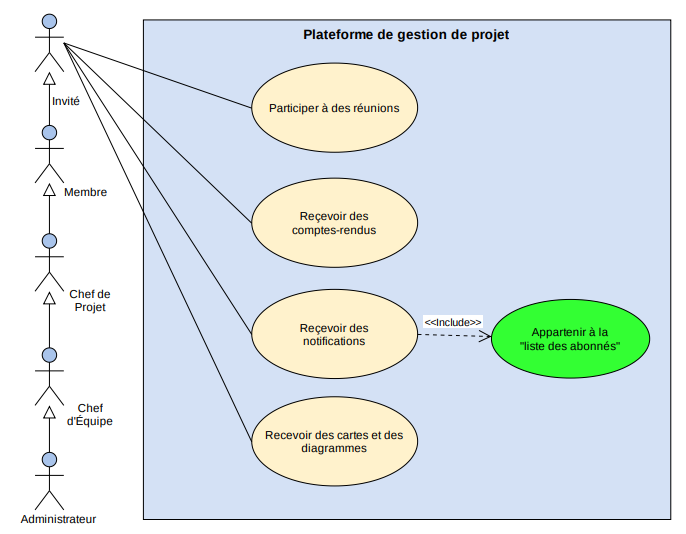
\includegraphics[scale=0.7]{figures/a4.png}
    \caption{Diagramme de cas d’utilisation pour l’invité}
    \label{fig:cas_invi}
\end{figure}
\newpage\par \textbf{	Membre :} cet acteur est un membre ajouté par l'administrateur qui a des missions à faire comme on peut le voir sur le diagramme (Figure \ref{fig:cas_memb}).

\begin{figure}[h]
    \centering
    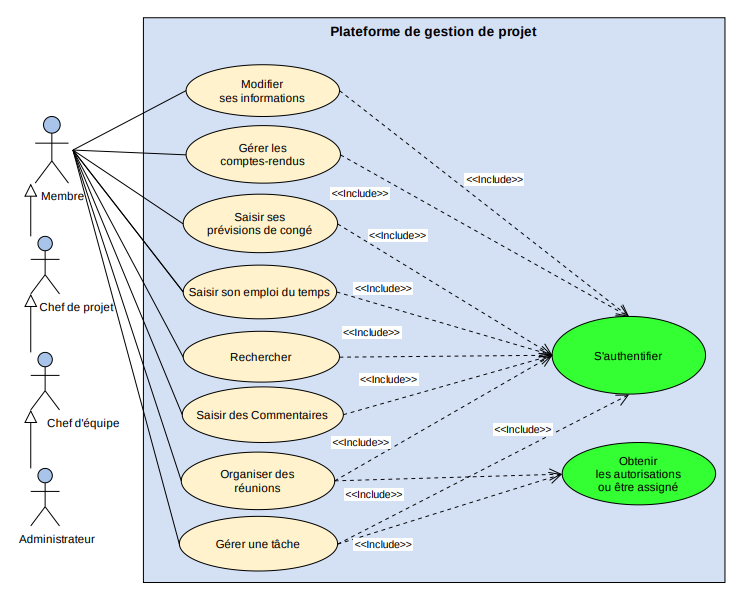
\includegraphics[scale=0.7]{figures/a9.png}
    \caption{Diagramme de cas d’utilisation pour un membre}
    \label{fig:cas_memb}
\end{figure}\newpage
\par \textbf{Chef de projet :} cet acteur est un chef de projet ajouté par l'administrateur qui a des missions à faire comme on peut le voir sur le diagramme (Figure \ref{fig:cas_chefp}).
\begin{figure}[h]
    \centering
    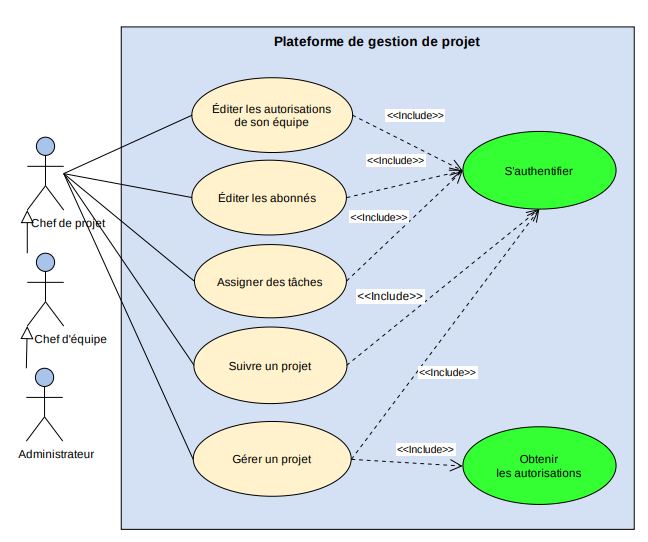
\includegraphics[scale=0.7]{figures/a1.png}
    \caption{Diagramme de cas d’utilisation pour le chef de projet}
    \label{fig:cas_chefp}
\end{figure}
\newpage
\par \textbf{	Chef d’équipe :} cet acteur est un chef d’équipe ajouté par l'administrateur qui a des missions à faire comme on peut le voir sur le diagramme (Figure \ref{fig:cas_chefe}).
\begin{figure}[h]
    \centering
    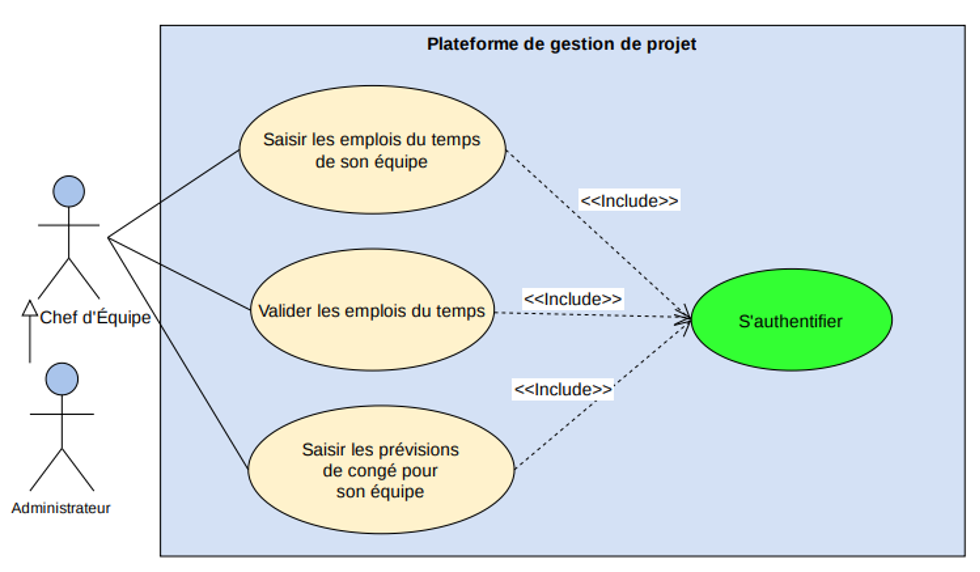
\includegraphics[scale=0.8]{figures/anis7.png}
    \caption{Diagramme de cas d’utilisation pour le chef d’équipe}
    \label{fig:cas_chefe}
\end{figure}

\par \textbf{ Administrateur :} cet acteur est un administrateur qui a des missions à faire comme on peut le voir sur le diagramme (Figure \ref{fig:cas_admin}).
\begin{figure}[h]
    \centering
    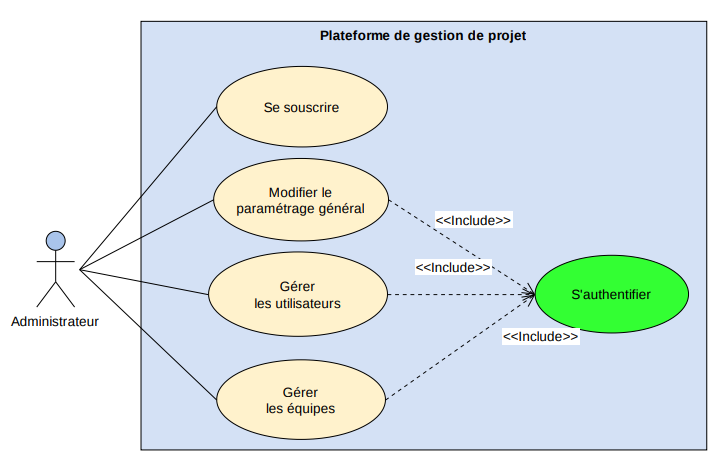
\includegraphics[scale=0.53]{figures/3333anis1.png}
    \caption{Diagramme de cas d’utilisation pour l’administrateur}
    \label{fig:cas_admin}
\end{figure}\newpage
\subsubsection{	Authentification}
\hspace{4mm}L’authentification est la condition préalable nécessaire à tous les autres processus décrits dans les diagrammes des cas d’utilisation. Elle doit être assurée pour permettre aux acteurs d’exécuter leurs propres cas d’utilisation. Le tableau ci-dessous décrit le processus d'authentification.
\begin{center}
\begin{tabular}{|c|l|}
\hline 
&\textbf { Description }\\\hline 
    Acteur principal & Utilisateur \\\hline 
    Objectif&L’utilisateur s’authentifie dans la plateforme.\\\hline
    Préconditions&Les données personnelles permettant l’authentification existent \\&dans la plateforme.\\\hline 
    Déclencheur&L’utilisateur ouvre la page d’authentification de la plateforme\\\hline 
    &Le système affiche un formulaire de login avec les champs email \\&d’utilisateur et mot de passe.\\
    Scénario nominal&L’utilisateur remplit les valeurs du formulaire et sélectionne \\&" Se connecter " une fois terminé.\\& Le système valide les données.\\
    &Le système permet à l’utilisateur de rentrer dans la plateforme.\\\hline
    &Le login échoue si : \\
    Extensions&le couple de valeurs email d’utilisateur + mot de passe ne se trouvent \\
    &pas dans la plateforme.\\\hline
\end{tabular}
\captionof{table}{Description du processus d’authentification}
\label{desc_auth}
\end{center}\newpage
\subsubsection{	Gestion des utilisateurs}
La figure \ref{fig:cas_gerutil} présente le diagramme de gestion de projet.
\begin{figure}[h]
    \centering
    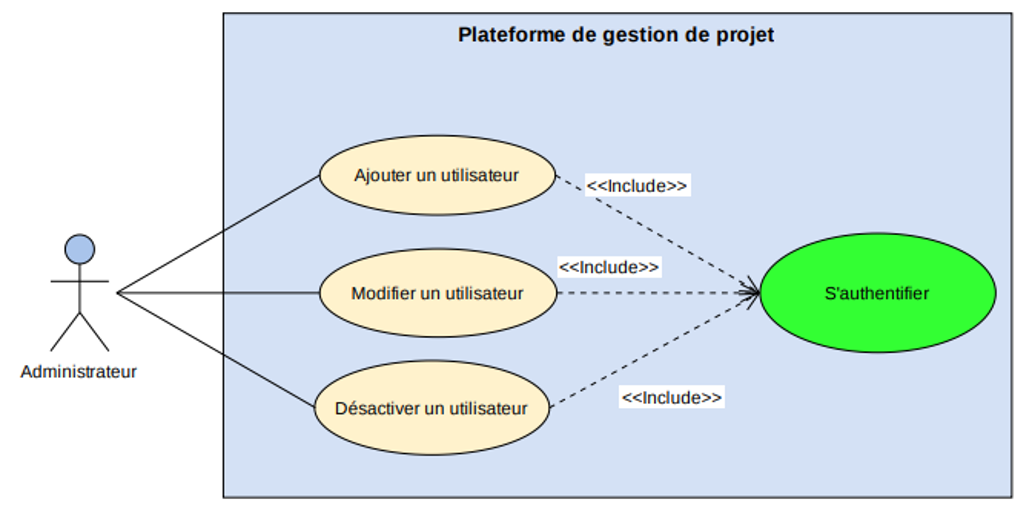
\includegraphics[scale=1]{figures/anis10.png}
    \caption{Diagramme de gestion des utilisateurs par l’administrateur}
    \label{fig:cas_gerutil}
\end{figure}
\par Dans la suite on va détailler les processus de gestion des utilisateurs par l’administrateur aux moyens de tableaux descriptifs.\newpage
\par \textbf{ 	Ajouter un utilisateur}
\par Le tableau suivant présente l’enchainement du cas d’utilisation "Ajouter un utilisateur"
\begin{center}
\begin{tabular}{|c|l|}
\hline 
&\textbf { Description }\\\hline 
    Acteur principal & Administrateur \\\hline 
    Objectif&L’administrateur doit pouvoir ajouter un utilisateur.\\\hline
    Préconditions&Il doit être authentifié.  \\&Il doit être administrateur.\\\hline 
    Déclencheur&L’administrateur choisit " Ajouter un utilisateur "\\\hline 
    &Le système affiche un formulaire d’ajout d’un utilisateur  \\& vide contenant les champs suivants : \\
    &Nom, prénom, email, mot de passe, équipe (liste à \\
    &choix d’équipe), rôle (liste à choix contenant Invité, membre,\\Scénario nominal&chef de projet, chef d’équipe, administrateur),liste des autorisations.\\
    &L’administrateur remplit les valeurs du formulaire \\
    & et sélectionne " enregistrer " une fois terminé.\\
    &Le système valide les données. \\
    &Le système enregistre l’utilisateur.  \\
    &Le système affiche le résultat : succès ou échec. \\\hline
    &L’enregistrement échoue si :  \\
    Extensions&les valeurs minimales ne sont pas remplies.  \\
    &un utilisateur avec ce mail existe déjà.\\\hline
\end{tabular}
\captionof{table}{Description du processus d'ajout d'un utilisateur}
\label{desc_ajout_ut}
\end{center}\newpage
\par \textbf{ 	Modifier un utilisateur}
\par Le tableau suivant présente l’enchainement du cas d’utilisation " Modifier un utilisateur "
\begin{center}
\begin{tabular}{|c|l|}
\hline 
&\textbf { Description }\\\hline 
    Acteur principal & Administrateur \\\hline 
    Objectif&L’administrateur doit pouvoir modifier un utilisateur.\\\hline
    Préconditions&Il doit être authentifié.  \\&Il doit être administrateur.\\\hline 
    Déclencheur&L’administrateur choisit un utilisateur "\\\hline 
    &Le système affiche le formulaire de l'utilisateur choisie   \\&contenant les champs suivants : \\
    &Nom, prénom, email, mot de passe, équipe (liste à \\
    &choix d’équipe), rôle (liste à choix contenant Invité, membre,\\Scénario nominal&chef de projet, chef d’équipe, administrateur).\\
    &L’administrateur remplit les valeurs du formulaire \\
    & et sélectionne " enregistrer " une fois terminé.\\
    &Le système valide les données. \\
    &Le système enregistre les modifications.   \\
    &Le système affiche le résultat : succès ou échec. \\\hline
    &L’enregistrement échoue si :  \\
    Extensions&les valeurs minimales ne sont pas remplies.  \\\hline
\end{tabular}
\captionof{table}{Description du processus de modification d'un utilisateur}
\label{desc_modif_ut}
\end{center}\newpage
\par \textbf{ 	 	Désactiver un utilisateur}
\par Le tableau suivant présente l'enchaînement du cas d'utilisation "désactiver un utilisateur".
\begin{center}
\begin{tabular}{|c|l|}
\hline 
&\textbf { Description }\\\hline 
    Acteur principal & Administrateur \\\hline 
    Objectif&L’administrateur doit pouvoir désactiver les données des utilisateurs.\\\hline
    Préconditions&Il doit être authentifié.  \\&Il doit être administrateur.\\\hline 
    Déclencheur&L’administrateur choisit un utilisateur de la liste des utilisateurs.\\\hline 
    &Le système affiche le formulaire de l’utilisateur choisi.    \\&L’administrateur choisit le bouton Désactiver.  \\
    Scénario nominal&Le système demande confirmation. \\
    &Le système valide la désactivation et l’exécute.  \\
    &Le système affiche le résultat : succès ou échec. \\\hline
    &La désactivation échoue si :   \\
    Extensions&l’utilisateur a fait des saisies des tâches ou des heures   \\
    &dans le système.\\\hline
\end{tabular}
\captionof{table}{Description du processus de désactivation d'un utilisateur}
\label{desc_desact_ut}
\end{center}\newpage
\subsubsection{	Gestion des équipes}
\hspace{4mm}La figure suivante présente le diagramme de gestion des équipes.
\begin{figure}[h]
    \centering
    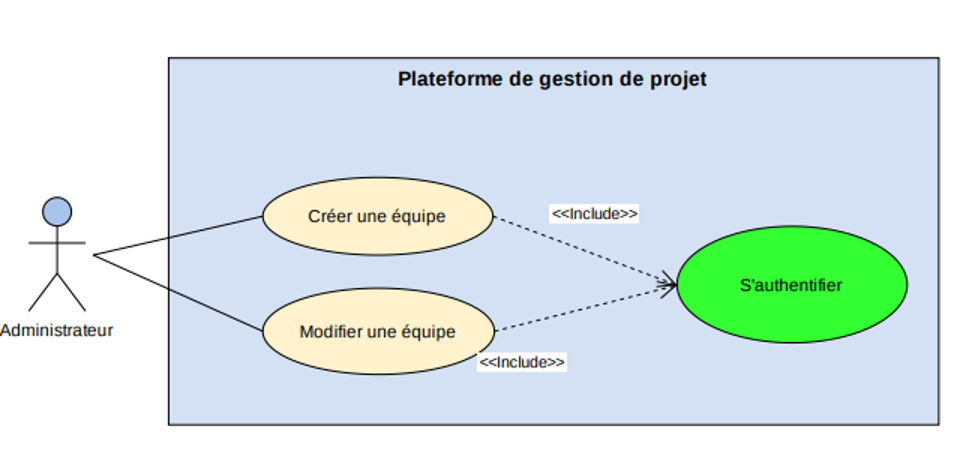
\includegraphics[scale=1]{figures/anis11.png}
    \caption{Diagramme de cas d'utilisation de la gestion des équipes par l’administrateur}
    \label{fig:cas_gereq}
\end{figure}
\par Dans la suite on va détailler les processus de gestion des équipes par l’administrateur aux moyens de tableaux descriptifs.
\newpage
\par \textbf{ 	Créer une équipe}
\par Le tableau suivant présente l'enchaînement du cas d'utilisation "créer une équipe".
\begin{center}
\begin{tabular}{|c|l|}
\hline 
&\textbf { Description }\\\hline 
    Acteur principal & Administrateur \\\hline 
    Objectif&L’administrateur doit pouvoir créer une équipe.\\\hline
    Préconditions&Il doit être authentifié.  \\&Il doit être administrateur.\\\hline 
    Déclencheur&L’administrateur choisit " Ajouter une équipe "\\\hline 
    &Le système affiche un formulaire d’ajout d’une équipe     \\&vide contenant les champs suivants :   \\
    &Nom de l’équipe, nom de projet (liste à choix), chef  \\
    &d’équipe (liste à choix), membres (liste à choix).\\
    &L’administrateur remplit les valeurs du formulaire et \\
    Scénario nominal&et sélectionne " enregistrer " une fois terminé.  \\
    &Le système valide les données. \\
    &Le système enregistre l'équipe. \\
    &Le système affiche le résultat : succès ou échec. \\
    &Le système envoie une notification à tous les utilisateurs \\&qui font partie de cette équipe.\\\hline
    &La désactivation échoue si :   \\
    Extensions&les valeurs minimales ne sont pas remplies.   \\
    &une équipe avec ce nom existe déjà.\\\hline
\end{tabular}
\captionof{table}{Description du processus d'ajout d'une équipe}
\label{desc_ajout_eq}
\end{center}\newpage
\par \textbf{ 	 	Modifier une équipe}
\par Le tableau suivant présente l’enchainement du cas d’utilisation "Modifier une équipe"
\begin{center}
\begin{tabular}{|c|l|}
\hline 
&\textbf { Description }\\\hline 
    Acteur principal & Administrateur \\\hline 
    Objectif&L’administrateur doit pouvoir modifier une équipe.\\\hline
    Préconditions&Il doit être authentifié.  \\&Il doit être administrateur.\\\hline 
    Déclencheur&L’administrateur choisit une équipe de la liste des équipes.\\\hline 
    &Le système affiche le formulaire de l'équipe choisie   \\&contenant les champs suivants :   \\
    &Nom de l’équipe, nom de projet (liste à choix),  \\
    &chef d’équipe (liste à choix), membre (liste à choix).\\
    &L’administrateur change les valeurs du formulaire et  \\
    Scénario nominal& sélectionne "enregistrer" une fois terminé.\\
    &Le système valide les données. \\
    &Le système enregistre les modifications.   \\
    &Le système affiche le résultat : succès ou échec. \\
    &Le système envoie une notification à tous les utilisateurs\\
    &qui font partie de cette équipe\\\hline
    Extensions&La modification échoue si :  \\
    &les valeurs minimales ne sont pas remplies. \\\hline
\end{tabular}
\captionof{table}{Description du processus de modification d'une équipe}
\label{desc_modif_eq}
\end{center}\newpage
\subsubsection{	Gestion de projet}
\par La figure suivante présente le diagramme de cas d’utilisation " Gestion de projet".
\begin{figure}[h]
    \centering
    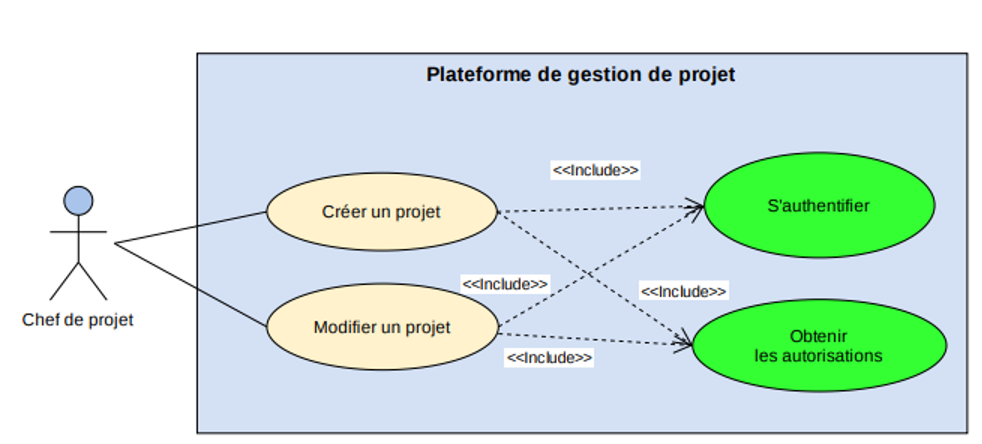
\includegraphics[scale=1]{figures/anis12.png}
    \caption{Diagramme de gestion de projet par le chef de projet}
    \label{fig:cas_gestp_chefp}
\end{figure}
\newpage
\par \textbf{ 	Création d’un projet}
\par Dans la suite on va détailler les processus de gestion de projet par le chef de projet aux moyens de tableaux descriptifs.
\begin{center}
\begin{tabular}{|c|l|}
\hline 
&\textbf { Description }\\\hline 
    Acteur principal & Chef de projet, chef d’équipe, Administrateur \\\hline 
    Objectif&Les acteurs doivent pouvoir créer un projet.\\\hline
    Préconditions&L’acteur doit être authentifié et doit avoir les autorisations.  \\\hline 
    Déclencheur&L’acteur choisit « Création de projet »\\\hline 
    &Le système affiche un formulaire de création de projet    \\&vide contenant les champs suivants :  \\
    &Nom de projet, date début, date fin, chef de projet   \\
    &(liste à choix des membres), description.\\
    Scénario nominal&L’acteur remplit les valeurs du formulaire et sélectionne   \\
    & " enregistrer " une fois terminé. \\
    &Le système valide les données. \\
    &Le système enregistre le projet.   \\
    &Le système affiche le résultat : succès ou échec. \\
    &Le système envoie une notification à tous les utilisateurs\\\hline
    &La modification échoue si :  \\
    Extensions&les valeurs minimales ne sont pas remplies.\\\hline
\end{tabular}
\captionof{table}{Description du processus de création d’un projet}
\label{desc_cree_proj}
\end{center}
\newpage
\par \textbf{ 	 	Modifier un projet}

\begin{center}
\begin{tabular}{|c|l|}
\hline 
&\textbf { Description }\\\hline 
    Acteur principal & Chef de projet, chef d’équipe, Administrateur \\\hline 
    Objectif&Les acteurs doivent pouvoir modifier un projet.\\\hline
    Préconditions&L’acteur doit être authentifié et doit avoir les autorisations.  \\\hline 
    Déclencheur&L’acteur choisit un projet de la liste des projets.\\\hline 
    &Le système affiche le formulaire de projet choisi    \\&contenant les champs suivants :  \\
    &Nom de projet, date début, date fin, chef de projet    \\
    &(liste à choix des membres), description.\\
    Scénario nominal&L’acteur modifier les valeurs du formulaire et sélectionne    \\
    & " enregistrer " une fois terminé. \\
    &Le système valide les données. \\
    &Le système enregistre le projet.   \\
    &Le système affiche le résultat : succès ou échec. \\
    &Le système envoie une notification à tous les utilisateurs\\\hline
    &La modification échoue si :  \\
    Extensions&les valeurs minimales ne sont pas remplies.\\\hline
\end{tabular}
\captionof{table}{Description du processus de modification d'un projet }
\label{desc_modif_proj}
\end{center}\newpage
\subsubsection{	Suivi de projet}
\hspace{4mm}La figure suivante présente le diagramme de cas d'utilisation " Suivi de projet".
\begin{figure}[h]
    \centering
    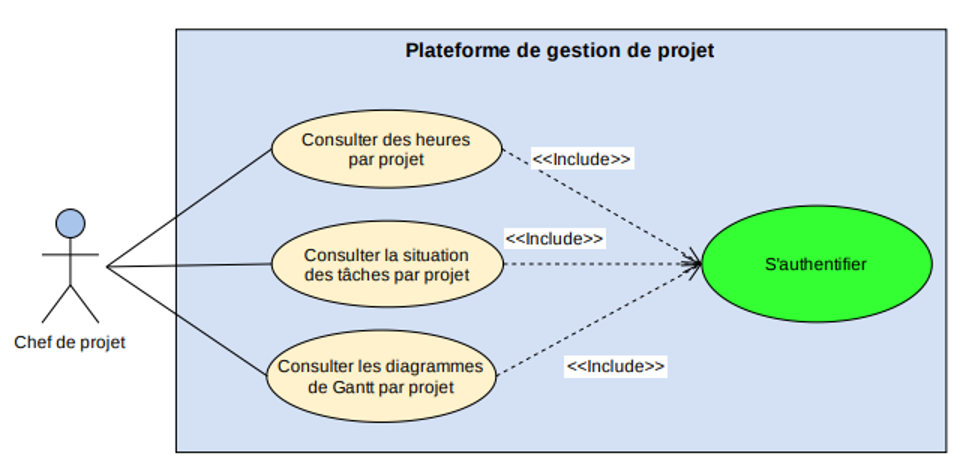
\includegraphics[scale=0.8]{figures/anis13.png}
    \caption{Diagramme de cas d'utilisation de suivi de projet par le chef de projet}
    \label{fig:cas_gestp_chefp}
\end{figure}
\par Dans la suite nous allons détailler les processus des differents cas d'utilisation qui correspondent au suivi de projet.
\par \textbf{  	Consultation des heures par projet	}
\par Ce service permet à certains acteurs de connaitre le nombre d'heures investies dans chaque projet.
\begin{center}
\begin{tabular}{|c|l|}
\hline 
&\textbf { Description }\\\hline 
    Acteur principal & Chef de projet, chef d’équipe, Administrateur \\\hline 
    Objectif&Les acteurs doivent pouvoir consulter les heures d’un projet.\\\hline
    Préconditions&L’acteur doit être authentifié.  \\\hline 
    Déclencheur&L’acteur choisit " Heures par projet "\\\hline 
    &Le système affiche un formulaire de recherche avec tous les projets.   \\
    &L’acteur remplit les valeurs du formulaire et sélectionne    \\
    Scénario nominal&" recherche " une fois terminé. \\
    &Le système effectue la recherche.    \\
    & Le système retourne les données recherchées sous forme de tableau  \\
    &dont toutes les colonnes peuvent être triées et filtrées.  \\\hline
    Extensions&                    - \\\hline
\end{tabular}
\captionof{table}{Description du processus de consultation des heures par projet}
\label{desc_cree_proj}
\end{center}
\newpage
\par \textbf{  	 	Consultation du diagramme de Gantt par projet	}
\par Le tableau suivant présente l’enchainement du cas d’utilisation " Consultation du diagramme de Gantt par projet "
\begin{center}
\begin{tabular}{|c|l|}
\hline 
&\textbf { Description }\\\hline 
    Acteur principal & Chef de projet, chef d’équipe, Administrateur \\\hline 
    Objectif&Les acteurs doivent pouvoir consulter le diagramme de Gantt par projet.\\\hline
    Préconditions&L’acteur doit être authentifié.  \\\hline 
    Déclencheur&L’acteur choisit "Consultation du diagramme de Gantt par projet"\\\hline 
    &Le système affiche un formulaire de recherche avec tous les projets.    \\
    &L'acteur remplit les valeurs du formulaire et sélectionne   \\
    Scénario nominal&" recherche " une fois terminé. \\
    &Le système effectue la recherche.    \\
    & Le système retourne le diagramme de Gantt qui correspond aux critères.   \\
    &Depuis ce diagramme, l’acteur doit pouvoir accéder aux tâches   \\
    &et les modifier.\\\hline
    Extensions&                    - \\\hline
\end{tabular}
\captionof{table}{Description du processus de consultation du diagramme de Gantt par projet}
\label{desc_diag_gantt}
\end{center}
\newpage
\par \textbf{  	 	 	Consultation de la situation des tâches par projet	}
\par Le tableau suivant présente l’enchainement du cas d’utilisation "Consultation de la situation des tâches par projet".
\begin{center}
\begin{tabular}{|c|l|}
\hline 
&\textbf { Description }\\\hline 
    Acteur principal & Chef de projet, chef d’équipe, Administrateur \\\hline 
    Objectif&Les acteurs doivent pouvoir consulter la situation des tâches par projet.\\\hline
    Préconditions&L’acteur doit être authentifié.  \\\hline 
    Déclencheur&L’acteur choisit "Consultation de la situation des tâche par projet"\\\hline 
    &Le système affiche un formulaire de recherche avec tous les projets     \\
    &et les états des tâches (A faire, En cours, Fait).   \\
    &Le chef de projet remplit les valeurs du formulaire et sélectionne  \\
    Scénario nominal&"recherche" une fois terminé.    \\
    & Le système effectue la recherche.   \\
    &Le système retourne les données recherchées sous forme de   \\
    &tableau dont toutes les colonnes peuvent être triées et filtrées.\\\hline
    Extensions&                    - \\\hline
\end{tabular}
\captionof{table}{Description du processus de consultation de la situation des tâches par projet}
\label{desc_tache_proj}
\end{center}
\newpage
\par \textbf{  	 	 	2.4.3.6	Editer les autorisations pour un autre membre	}
\par Tout acteur de type chef d’équipe, chef de projet ou administrateur, dépendamment de son niveau, peut changer les types d'accès du reste des membres de l'équipe qu'il gère.
\par Le tableau ci-dessous décrit le processus d'édition des autorisations pour un autre membre.
\begin{center}
\begin{tabular}{|c|l|}
\hline 
&\textbf { Description }\\\hline 
    Acteur principal & Chef de projet, chef d’équipe, Administrateur \\\hline 
    Objectif&Les acteurs doivent pouvoir éditer les autorisations pour un autre membre.\\\hline
    Préconditions&L’acteur doit être authentifié.  \\\hline 
    Déclencheur&L’acteur choisit un membre de la liste des membres.\\\hline 
    &Le système affiche le formulaire du membre choisi contenant les champs     \\&suivants :\\
    &Nom, prénom, email, mot de passe, équipe, rôle, liste d’autorisation.   \\
    &L’acteur change les valeurs de la liste d'autorisation et sélectionne   \\
    Scénario nominal&" enregistrer " une fois terminé.   \\
    & Le système valide les données.    \\
    &Le système enregistre les modifications.   \\
    &Le système affiche le résultat : succès ou échec.\\
    &Le système envoie une notification d’information à ce membre.\\\hline
      &La modification échoue si :  \\
    Extensions&les valeurs minimales ne sont pas remplies.\\\hline             
\end{tabular}
\captionof{table}{Description du processus d'edition des autorisations pour un autre membre}
\label{desc_edit_autor}
\end{center}
\newpage
\subsubsection{		Gestion des tâches}
\hspace{4mm}La figure suivante présente le diagramme de cas d'utilisation " Gestion des tâches "
\begin{figure}[h]
    \centering
    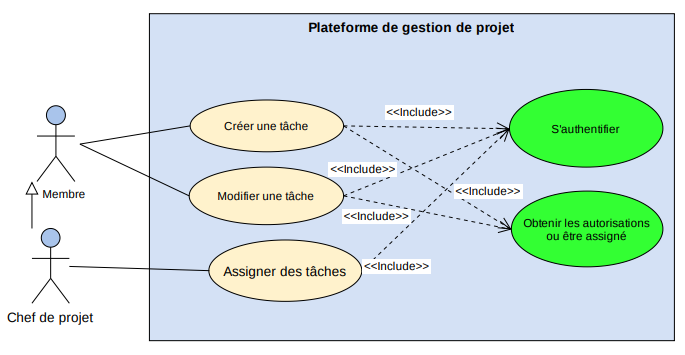
\includegraphics[scale=0.63]{figures/a3.png}
    \caption{Diagramme de cas d'utilisation de gestion des tâches par un membre }
    \label{fig:cas_gerer_tache}
\end{figure}
\par Dans la suite nous allons détailler les processus des différents cas d'utilisations qui correspondent de la gestion des tâches par un membre.
\newpage
\par \textbf{  	 	Création d’une tâche	}
\par Le tableau suivant présente la description du cas d'utilisation de création d'une tâche.
\begin{center}
\begin{tabular}{|c|l|}
\hline 
&\textbf { Description }\\\hline 
    Acteur principal & Chef de projet, chef d’équipe, Administrateur \\\hline 
    Objectif&Les acteurs doivent pouvoir créer une tâche.\\\hline
    Préconditions&L’acteur doit être authentifié et doit avoir les autorisations.  \\\hline 
    Déclencheur&L’acteur choisit " Nouvelle tâche "\\\hline 
    &Le système affiche un formulaire de nouvelle activité vide avec     \\
    &les champs suivants :    \\
    &Sujet, description, date début, date de fin, responsable (liste  \\
    Scénario nominal&à choix des membres), projet (liste à choix des projets).    \\
    & L’acteur remplit le formulaire.  \\
    &Le système valide les données. \\&Le système enregistre la tâche. \\&Le système affiche le résultat : succès ou échec.  \\\hline
    Extensions&La tâche ne peut pas être ajoutée si : \\&les valeurs minimales ne sont pas remplies.\\\hline
\end{tabular}
\captionof{table}{Description du processus de création d’une tâche}
\label{desc_cree_tache}
\end{center}
\newpage
\par \textbf{  	 	 	Assignation et modification des tâches	}
\par Le tableau suivant présente la description du cas d'utilisation de l’assignation et modification des tâches.
\begin{center}
\begin{tabular}{|c|l|}
\hline 
&\textbf { Description }\\\hline 
    Acteur principal & Chef de projet, chef d’équipe, Administrateur \\\hline 
    Objectif&Les acteurs doivent pouvoir assigner les tâches.\\\hline
    Préconditions&L’acteur doit être authentifié et doit avoir les autorisations.  \\\hline 
    Déclencheur&L’acteur choisit "Rechercher une tâche"\\\hline 
    &Le système affiche les paramètres de recherche suivants :      \\
    &Projet, utilisateur, état de l’activité (A Faire, En cours, Fait, Tout).   \\
    &L’acteur choisit ses paramètres et lance la recherche  \\
    Scénario nominal&Le système génère une " Vue " avec toutes les tâches     \\
    & correspondant à la recherche.   \\&L’acteur choisit la tâche qui l’intéresse et l’assigne à un membre.\\
    &Le système valide les données. \\&Le système enregistre la tâche. \\&Le système envoie une notification au membre assigné.\\&Le système affiche le résultat : succès ou échec.  \\\hline
    Extensions&   -\\\hline
\end{tabular}
\captionof{table}{Description du processus d'assignation et modification des tâches}
\label{desc_modif_tache}
\end{center}
\newpage
\par \textbf{  	 	Organiser des réunions	}
\par Le tableau suivant présente l’enchainement du cas d’utilisation "Organiser des réunions".
\begin{center}
\begin{tabular}{|c|l|}
\hline 
&\textbf { Description }\\\hline 
    Acteur principal & Chef de projet, chef d’équipe, Administrateur \\\hline 
    Objectif&Les acteurs doivent pouvoir organiser une réunion.\\\hline
    Préconditions&L’acteur doit être authentifié.  \\\hline 
    Déclencheur&L’acteur choisit " Nouvelle réunion "\\\hline 
    &Le système affiche un formulaire de nouvelle réunion vide       \\
    &avec les champs suivants :    \\
    &Organisateur, Objet, description, horaire/date, participants   \\
    Scénario nominal&(liste à choix des membres), emplacement.     \\
    & L’acteur remplit le formulaire.    \\
    &Le système valide les données. \\&Le système enregistre la réunion.  \\&Le système affiche le résultat : succès ou échec.  \\\hline
    Extensions&  La réunion ne peut pas être ajoutée si : \\&les valeurs minimales ne sont pas remplies.\\\hline
\end{tabular}
\captionof{table}{Description du processus d'organisation des réunions}
\label{desc_org_reunion}
\end{center}
\newpage
\par \textbf{  	Saisie emploi du temps	}
\par Le tableau suivant présente l’enchainement du cas d’utilisation "Saisie emploi du temps".
\begin{center}
\begin{tabular}{|c|l|}
\hline 
&\textbf { Description }\\\hline 
    Acteur principal & Chef de projet, chef d’équipe, Administrateur \\\hline 
    Objectif&Les acteurs doivent pouvoir saisir leurs emplois du temps.\\\hline
    Préconditions&L’acteur doit être authentifié.  \\\hline 
    Déclencheur&L’acteur choisit "Saisie emploi du temps"\\\hline 
    &L’utilisateur choisit le projet, la tâche, la date, la description       \\
    &et le nombre d’heures.     \\
    Scénario nominal&L’utilisateur soumet les valeurs au serveur.   \\
    &Le serveur valide les données, les enregistre et retourne le résultat    \\
    & à l’utilisateur : succès ou échec.   \\
    \hline
    Extensions&  L'emploi du temps ne peut pas être ajoutée si : \\&les valeurs minimales ne sont pas remplies.\\\hline
\end{tabular}
\captionof{table}{Description du processus de saisie de l'emploi du temps}
\label{desc_emp_temps}
\end{center}

\subsubsection{		Gestion des comptes rendus}
\hspace{4mm}La figure suivante présente le diagramme de cas d'utilisation "Gérer les comptes rendus"
\begin{figure}[h]
    \centering
    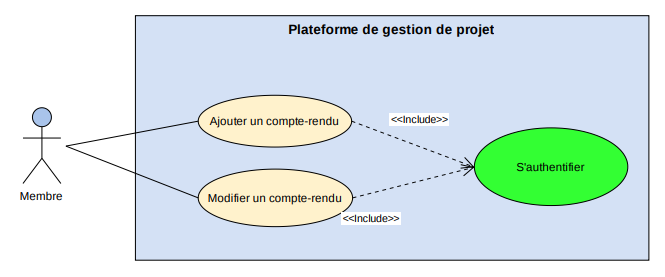
\includegraphics[scale=0.65]{figures/a2.png}
    \caption{Diagramme de cas d'utilisation de gestion des comptes rendus par un membre }
    \label{fig:cas_gerer_cmpterendu}
\end{figure}
\par Dans la suite nous allons détailler les processus des différents cas d'utilisations qui correspondent à la gestion des comptes rendus.
\par \textbf{  	 	 	 	Ajouter un compte-rendu	}
\par Le tableau suivant présente l’enchainement du cas d’utilisation "Ajouter un compte rendu".
\begin{center}
\begin{tabular}{|c|l|}
\hline 
&\textbf { Description }\\\hline 
    Acteur principal & Chef de projet, chef d’équipe, Administrateur \\\hline 
    Objectif&Les acteurs doivent pouvoir ajouter un compte-rendu.\\\hline
    Préconditions&L’acteur doit être authentifié.  \\\hline 
    Déclencheur&L’acteur choisit " Ajouter un compte-rendu "\\\hline
    &Le système affiche un formulaire de nouveau compte-rendu   \\
    &vide avec les champs suivants :    \\
    &Réunion (liste à choix des réunions), description (elle regroupe  \\
    &les points déjà mentionnés dans l’invitation à la réunion avec la      \\
    Scénario nominal& possibilité d’ajouter des points supplémentaires), participants    \\&(liste à choix des utilisateurs).\\&L’acteur remplit le formulaire. \\
    &Le système valide les données. \\&Le système enregistre le compte-rendu.  \\&Le système affiche le résultat : succès ou échec.  \\&Le système envoie une notification aux utilisateurs participants.\\\hline
    Extensions&   L’enregistrement échoue si :\\&les valeurs minimales ne sont pas remplies.\\\hline
\end{tabular}
\captionof{table}{Description du processus de gestion des comptes rendus}
\label{desc_gerer_cmpterendu}
\end{center}
\newpage
\par \textbf{  	Modifier un compte-rendu	}
\par Le tableau suivant présente l’enchainement du cas d’utilisation "Modifier un compte rendu".
\begin{center}
\begin{tabular}{|c|l|}
\hline 
&\textbf { Description }\\\hline 
    Acteur principal & Chef de projet, chef d’équipe, Administrateur \\\hline 
    Objectif&Les acteurs doivent pouvoir modifier un compte-rendu.\\\hline
    Préconditions&L’acteur doit être authentifié.  \\\hline 
    Déclencheur&L’acteur choisit un compte-rendu de la liste des comptes rendus.\\\hline
    &Le système affiche le formulaire du compte-rendu choisi    \\
    &contenant les champs suivants :    \\
    &Réunion (liste à choix des réunions), description (elle regroupe  \\
    &les points déjà mentionnés dans l’invitation à la réunion avec la      \\
    Scénario nominal& possibilité d’ajouter des points supplémentaires), participants    \\&(liste à choix des utilisateurs).\\&L’acteur modifie le formulaire. \\
    &Le système valide les données. \\&Le système enregistre les modifications apportées au compte-rendu.  \\&Le système affiche le résultat : succès ou échec.  \\&Le système envoie une notification aux utilisateurs participants.\\\hline
    Extensions&   L’enregistrement échoue si :\\&les valeurs minimales ne sont pas remplies.\\\hline
\end{tabular}
\captionof{table}{Description du processus de modification des comptes rendus}
\label{desc_modif_cmpterendu}
\end{center}
\newpage
\subsubsection{	Saisie de prévision de congé	}
\par Le tableau suivant présente l’enchainement du cas d’utilisation "Saisie prévision de congé".
\begin{center}
\begin{tabular}{|c|l|}
\hline 
&\textbf { Description }\\\hline 
    Acteur principal & Chef de projet, chef d’équipe, Administrateur \\\hline 
    Objectif&Les acteurs doivent pouvoir saisir leurs prévisions de congé.\\\hline
    Préconditions&L’acteur doit être authentifié.  \\\hline 
    Déclencheur&L’acteur choisit "Saisie prévision de congé"\\\hline
    &Le système affiche un formulaire de nouvelle prévision de congé\\
    &vide avec les champs suivants :    \\
    &Date début, date fin.   \\
   &L’acteur remplit le formulaire.  \\
    &Le système valide les données. \\&Le système enregistre la prévision de congé. \\&Le système affiche le résultat : succès ou échec.  \\&Le système envoie une notification à l’administrateur.\\\hline
    Extensions&   L’enregistrement échoue si :\\&les valeurs minimales ne sont pas remplies.\\\hline
\end{tabular}
\captionof{table}{Description du processus de saisie de prévision de congé}
\label{desc_saisie_conge}
\end{center}


\section*{Conclusion}
\hspace{4mm} Ce chapitre nous a permis de présenter les besoins fonctionnels de l’utilisateur et de définir les besoins non fonctionnels à prendre en considération afin de le satisfaire les utilisateurs et de détailler les cas d’utilisation de notre plateforme. La spécification des besoins étant établie, le chapitre suivant présentera une conception claire de l’architecture de la
plateforme proposée.  

\chapter{Conception } \label{ch:conc}


\hspace{4mm} La modélisation a pour objectif de formaliser les étapes préliminaires du développement d'un système afin de répondre aux besoins fixés dans la spécification du système. 
\par Dans ce chapitre nous détaillons les points forts de l’UML, par la suite nous présentons une conception détaillée pour bien comprendre la structure de notre projet. 
\section{	Architecture de l'application  }

\hspace{4mm} Afin de simplifier la mise à jour de l’application et d’en faciliter l’accès, le futur système va être développé sur la base d’une application Web. Une application Web se trouve sur un serveur et se manipule à l'aide d'un navigateur Web (Chrome, Firefox, …), via un réseau informatique (Internet, intranet, réseau local, etc.). Dans la technologie client-serveur, utilisée pour le World Wide Web, la communication est organisée par l'intermédiaire d'un réseau et d'une interface Web entre plusieurs ordinateurs." cela signifie que des machines clientes (machines faisant partie du réseau) contactent un serveur, une machine généralement très puissante en termes de capacités d'entrées-sorties, qui leur fournit des services. Ces services sont exploités par des programmes, appelés programmes clients, s'exécutant sur les machines clientes."\cite{12}.  
\par L'application Web s'oriente autour d'un serveur Web sur lequel est branché le logiciel applicatif, le tout accompagné d'un serveur de base de données.  
\par 
	Un des principaux avantages d’une application Web est que son utilisation est totalement indépendante du matériel de l’utilisateur. Qu’il utilise un PC ou un autre environnement, l’utilisateur n'a besoin que d’un explorateur pour accéder au système.


\subsection{	Design pattern MVC    }


\hspace{4mm}Dans le souci de développer une application stable et évolutive, l’utilisation d’une architecture standardisée est primordiale. Le Design Pattern Model-View-Controller est l'une des techniques de codage les plus répandues, principalement dans le développement Web. Les nouvelles possibilités d’interfaçages riches apportent de nouveaux défis. Le pattern MVC offre la possibilité de créer des applications plus flexibles. 
\par Rassembler les vues et les données a plusieurs inconvénients : 
\begin{itemize}
    \item 	La difficulté de gérer les données de l’extérieur de l’objet. 
    \item	La difficulté de créer différentes interfaces utilisateurs. 
    \item 	La difficulté de faire évoluer les interfaces. 
\end{itemize}
\par  Le concept de base du pattern MVC repose sur la séparation des données et des vues dans des logiques différentes. Le pattern MVC est basé sur trois couches : 
\par\textbf{	Le modèle }

\par Il décrit ou contient les données manipulées par l'application. Dans le cas typique d'une base de données le modèle offre des méthodes pour mettre à jour ces données (insertion, suppression, changement de valeur). Il offre aussi des méthodes pour récupérer ces données. Les résultats renvoyés par le modèle sont dénués de toute présentation. C'est le modèle qui contient toute la logique métier de l'application \cite{2}. 
\par\textbf{	La vue  }

\par La vue correspond à l'interface avec laquelle l'utilisateur interagit. Sa première tâche est de présenter les résultats renvoyés par le modèle qui lui sont passés par le contrôleur. Sa seconde tâche est de recevoir toutes les actions de l'utilisateur (clic de souris, sélection d'une entrée, boutons, soumission de formulaires). Ces différents événements sont envoyés au contrôleur. La vue n'effectue aucun traitement, elle se contente d'afficher les résultats des traitements effectués par le modèle \cite{2}. 
\newpage \par \textbf{	Le contrôleur   }

\par Le contrôleur prend en charge la gestion des événements de synchronisation pour mettre à jour la vue ou le modèle et les synchroniser. Il reçoit tous les événements de l'utilisateur et dénclenche les actions à effectuer. Si une action nécessite un changement des données, le contrôleur demande la modification des données au modèle et ensuite avertit la vue que les données ont changé pour qu'elle se mette à jour \cite{2}.
\begin{figure}[h]
    \centering
    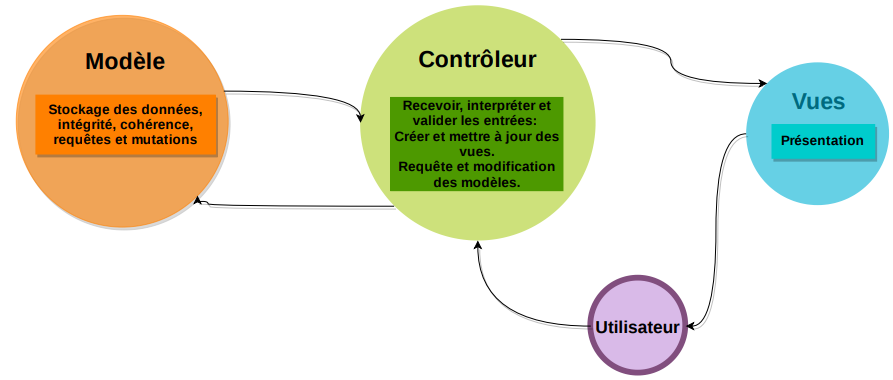
\includegraphics[scale=0.5]{figures/a11.png}
    \caption{Architecture MVC}
    \label{fig:Arch_MVC}
\end{figure}
\par En résumé, lorsqu'un client envoie une requête à l'application :
\begin{itemize}
    \item 	La requête est analysée par le contrôleur. 
    \item Le contrôleur demande au modèle approprié d'effectuer les traitements.
    \item 	Le contrôleur renvoie la vue adaptée. 
\end{itemize}

\subsection{	Backend Spring Boot avec Spring Security }
\hspace{4mm}Voici un diagramme pour les classes Spring Security / JWT qui sont séparées en 3 couches \cite{3}:
\begin{itemize}
    \item 	HTTP
    \item 	Spring Security
    \item 	REST API
\end{itemize}
\newpage
\begin{figure}[h]
    \centering
    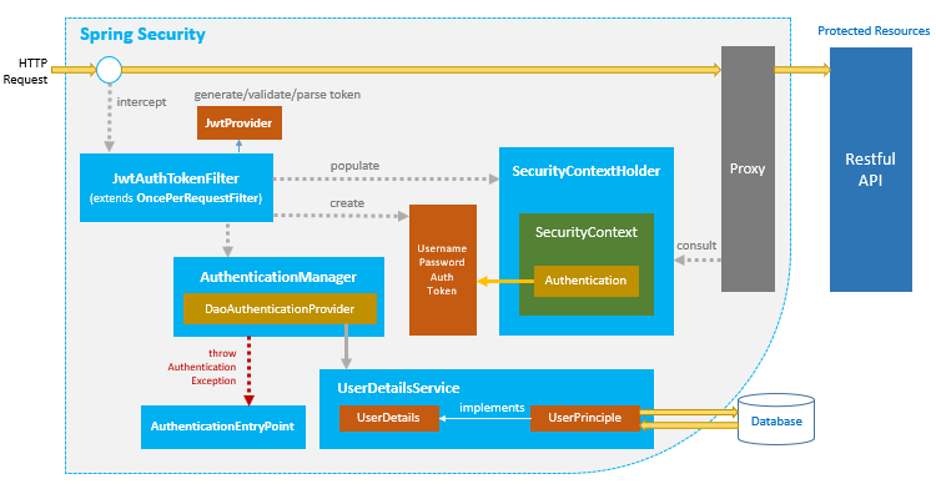
\includegraphics{figures/3anis1.png}
    \caption{Architecture Backend Spring Boot avec Spring Security \cite{3}}
    \label{fig:arch_backend}
\end{figure}
\begin{itemize}
    \item[-]\textbf{SecurityContextHolder} permet d'accéder au \textbf{SecurityContext}.
    \item[-] \textbf{SecurityContext} contient l'authentification et éventuellement les informations de sécurité spécifiques à la demande.
    \item[-]	L'authentification appelle \textbf{UserPrinciple} qui inclut \textbf{GrantedAuthority} qui reflète les autorisations à l'échelle de l'application accordée à \textbf{UserPrinciple}.
    \item[-]\textbf{UserDetails} contient les informations nécessaires pour créer un objet d'authentification à partir de DAO ou d'une autre source de données de sécurité.
    \item[-]\textbf{UserDetailsService} permet de créer un \textbf{UserDetails} à partir d'un nom d'utilisateur basé sur une chaîne et est généralement utilisé par \textbf{AuthenticationProvider}.
    \item[-]\textbf{JwtAuthTokenFilter} (étend \textbf{OncePerRequestFilter}) prétraite la requête HTTP, à partir de Token, crée une \textbf{Authentification} et la remplit dans \textbf{SecurityContext}.
    \item[-]\textbf{JwtProvider} valide, analyse la chaîne de jeton ou génère la chaîne de jeton à partir de \textbf{UserDetails}.
    \item[-]\textbf{UsernamePasswordAuthenticationToken} obtient l’email/ mot de passe de la demande de connexion et se combine dans une instance de l'interface d'authentification.
    \item[-]\textbf{AuthenticationManager} utilise \textbf{DaoAuthenticationProvider} (avec l'aide de \textbf{UserDetailsService et PasswordEncoder}) pour valider l'instance de \textbf{UsernamePasswordAuthenticationToken}, puis renvoie une instance d'authentification entièrement remplie en cas d'authentification réussie.
    \item[-]\textbf{SecurityContext} est établi en appelant \newline \textbf{SecurityContextHolder.getContext().SetAuthentication(…)} avec l'objet d'authentification renvoyé ci-dessus.
    \item[-]\textbf{AuthenticationEntryPoint} gère \textbf{AuthenticationException}.
    \item[-]L'accès à Restful API est protégé par HTTPSecurity et autorisé avec Method Security Expressions.
\end{itemize}
\subsection{	Front-end angular avec interceptor }
\hspace{4mm}La figure \ref{fig:arch_frontend} ci-dessous décrit l'architecture angular avec interceptor. \cite{4}
\begin{figure}[h]
    \centering
    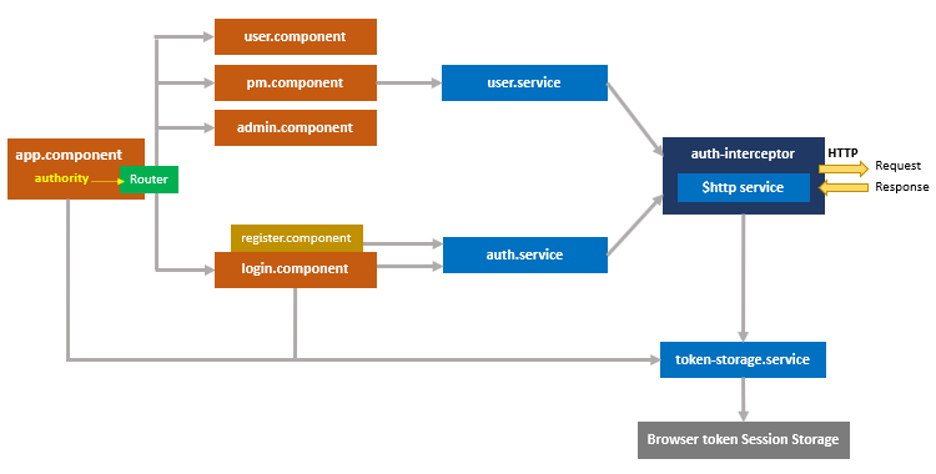
\includegraphics{figures/3anis2.png}
    \caption{Architecture Front-end angular avec interceptor \cite{4}}
    \label{fig:arch_frontend}
\end{figure}
\begin{itemize}
    \item[-]\textbf{app.component} est le composant parent qui contient \textbf{routerLink} et \textbf{router-outlet} pour le routage. Il a également une variable d'autorité comme condition d'affichage des éléments sur la barre de navigation. 
e    \item[-]\textbf{user.component, pm.component} et  \textbf{admin.component} correspondent à Angular Components for User Board, PM Board et Admin Board. Chaque conseil utilise \textbf{user.service} pour accéder aux données d'autorité.
    \item[-]\textbf{register.component} contient le formulaire d'inscription de l'utilisateur, la soumission du formulaire appellera \textbf{auth.service}.
    \item[-]\textbf{login.component} contient le formulaire de connexion utilisateur, la soumission du formulaire appellera \textbf{auth.service} et \textbf{token-storage.service}.
    \item[-]\textbf{user.service} obtient l'accès aux données d'autorité du serveur en utilisant Angular \textbf{HttpClient} (http service).
    \item[-]Chaque requête HTTP par le service \textbf{http} sera inspectée et transformée avant d'être envoyée au serveur par auth-interceptor (implements \textbf{HttpInterceptor}).
    \item[-]\textbf{auth-interceptor} vérifie et récupère le jeton depuis \textbf{token-storage.service} pour ajouter le jeton à l'en-tête d'autorisation des requêtes HTTP.
    \item[-]\textbf{token-storage.service} gère le jeton dans le sessionStorage du navigateur.
\end{itemize}
\subsection{	Architecture angular 9 et Spring Boot}
\hspace{4mm}La figure \ref{fig:spring_boot} ci-dessous décrit l'architecture angular et spring boot:
\begin{figure}[h]
    \centering
    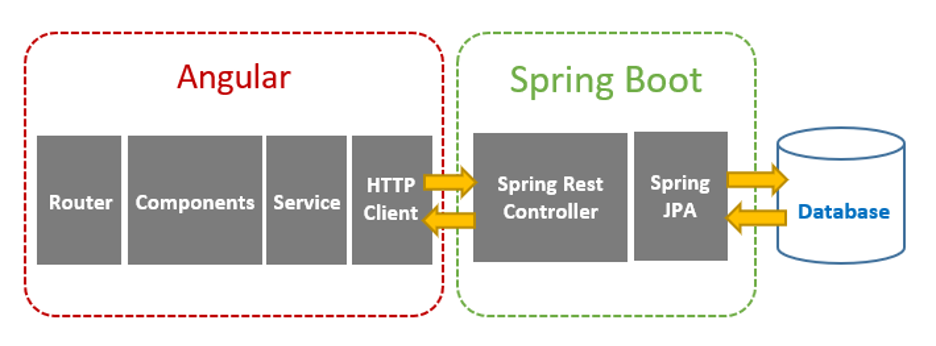
\includegraphics{figures/3anis3.png}
    \caption{Architecture angular 9 ET Spring Boot \cite{13}}
    \label{fig:spring_boot}
\end{figure}
\begin{itemize}
    \item	Spring Boot exporte les Apis REST à l'aide de Spring Web MVC et interagit avec la base de données à l'aide de Spring Data JPA.
    \item Angular Client envoie des requêtes HTTP, récupère des réponses HTTP et affiche des données sur les composants. Nous utilisons également Angular Router pour accéder aux pages.
    \item 	La base de données est PostgreSQL.
\end{itemize}
\section{Conception détaillée}
\subsection{	Diagrammes de classes }
\subsubsection{	Diagramme de classes global}
\hspace{4mm}Les classes font partie de la logique de l’application. Elles présentent non seulement la structure statique, mais aussi les différentes entités qui sont invoquées dans la conception de notre application. La figure \ref{fig:class_global} suivante présente le diagramme de classes que nous avons utilisé tout au long de ce projet. Les classes que nous avons créées dans ce projet correspondent à celles qui sont colorées dans la figure ci-dessous.
\par Dans la figure \ref{fig:class_global} on observe le diagramme de classe général en détails, à voir :
\begin{itemize}
    \item 	La classe : est un concept abstrait qui permet de représenter toutes les entités d'un système.
    \item	Les champs : ayant un type, pour distinguer le type de données à stocker pour ce champ.
    \item	La liaison d’héritage : Démarche ascendante, qui consiste à capturer les particularités communes d'un ensemble d'objets, issus de classes différentes.
    \item	La liaison d’agrégation : est une association non symétrique, qui exprime un couplage fort et une relation de subordination. Elle représente une relation de type "ensemble / élément".
    \item 	Les cardinalités de chaque liaison : selon le besoin, on distingue trois types de cardinalité sous django : 
    \begin{itemize}
        \item  ManyToMany relation : relation forte.
        \item  ManyToOne relation : relation moyenne
        \item  OneToOne relation : relation faible
    \end{itemize}
\end{itemize}


\begin{figure}
    \centering
    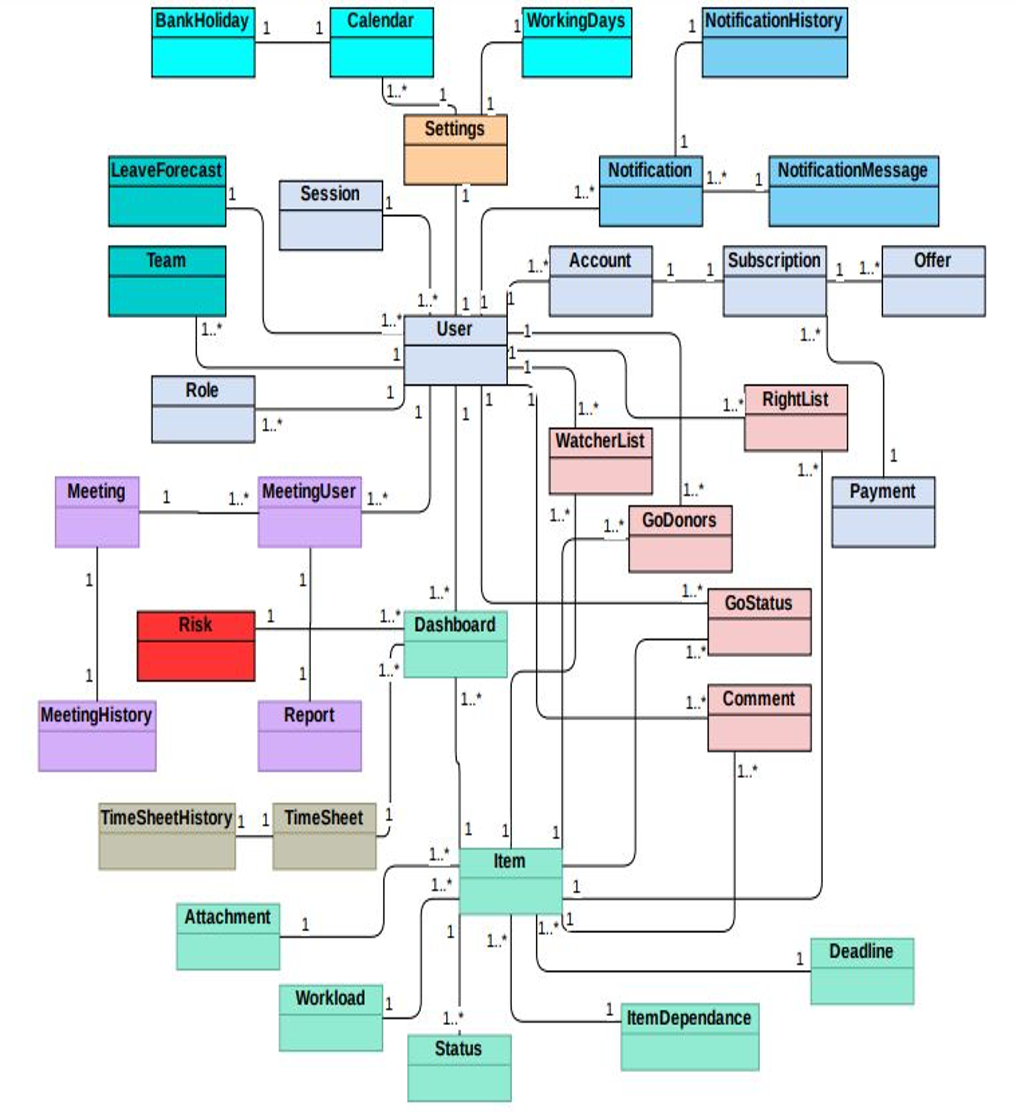
\includegraphics{figures/33anis.png}
    \caption{Diagramme de classes globale}
    \label{fig:class_global}
\end{figure}
\newpage
\subsubsection{	Diagramme de classes «Inscription et Authentification  »}
\hspace{4mm}Dans le diagramme de la figure \ref{fig:class_auth} on détaille les classes ainsi que les liaisons entre elles  pour la partie inscription et authentification.
\begin{itemize}
    \item 	Avant de s’inscrire (soumission des données d’un formulaire d’inscription) un objet de la classe \textbf{Session} est crée, il fournit en plus de son Id  un Token qui sera renvoyé par la suite à l’utilisateur dans le but de vérifier le statut de l’utilisateur (\textbf{status} :" True " peut se connecter, " False " connexion au compte impossible) avec un attribut lastConnection précisant un délai pour lequel le Token est valable.
    \item 	Saisie d’une offre : l’utilisateur choisit une offre de son choix tout en précisant le type de payement.  
\end{itemize}
\begin{figure}[h]
    \centering
    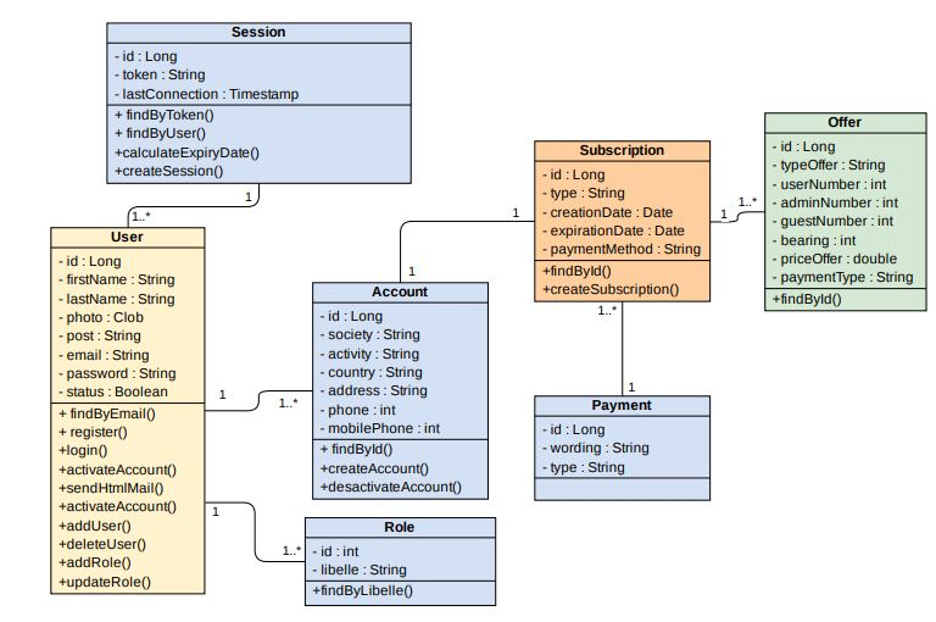
\includegraphics{figures/33Anis1.png}
    \caption{Diagramme de classes « Inscription et Authentification  »}
    \label{fig:class_auth}
\end{figure}\newpage
\subsubsection{Diagramme de classes « Gestion des Réunions, Notifications, Équipe et Paramétrage  »}
\begin{itemize}
    \item \textbf{Réunions} : En plus des détails des \textbf{Meeting} on trouve la classe \textbf{MeetingHistory} qui sert pour le traçage  des anciennes réunions établies via la plateforme ainsi qu’une classe Report qui permettra d’obtenir un compte Rendu de la réunion.
    \item \textbf{Notifications}: le contenu de la notification est récupéré par la classe \textbf{NotificationMessage}. Toute notification admet un statut et dispose d’un historique.
    \item \textbf{Paramétrage} : le paramétrage permet de donner les jours des travaux (on trouve les jours de la semaine qui sont bien partitionnés). On peut préciser les jours de congé en suivant la classe calendrier.
	\item\textbf{Équipe} : un utilisateur peut appartenir à une équipe.
\end{itemize}\newpage
\begin{figure}[h]
    \centering
    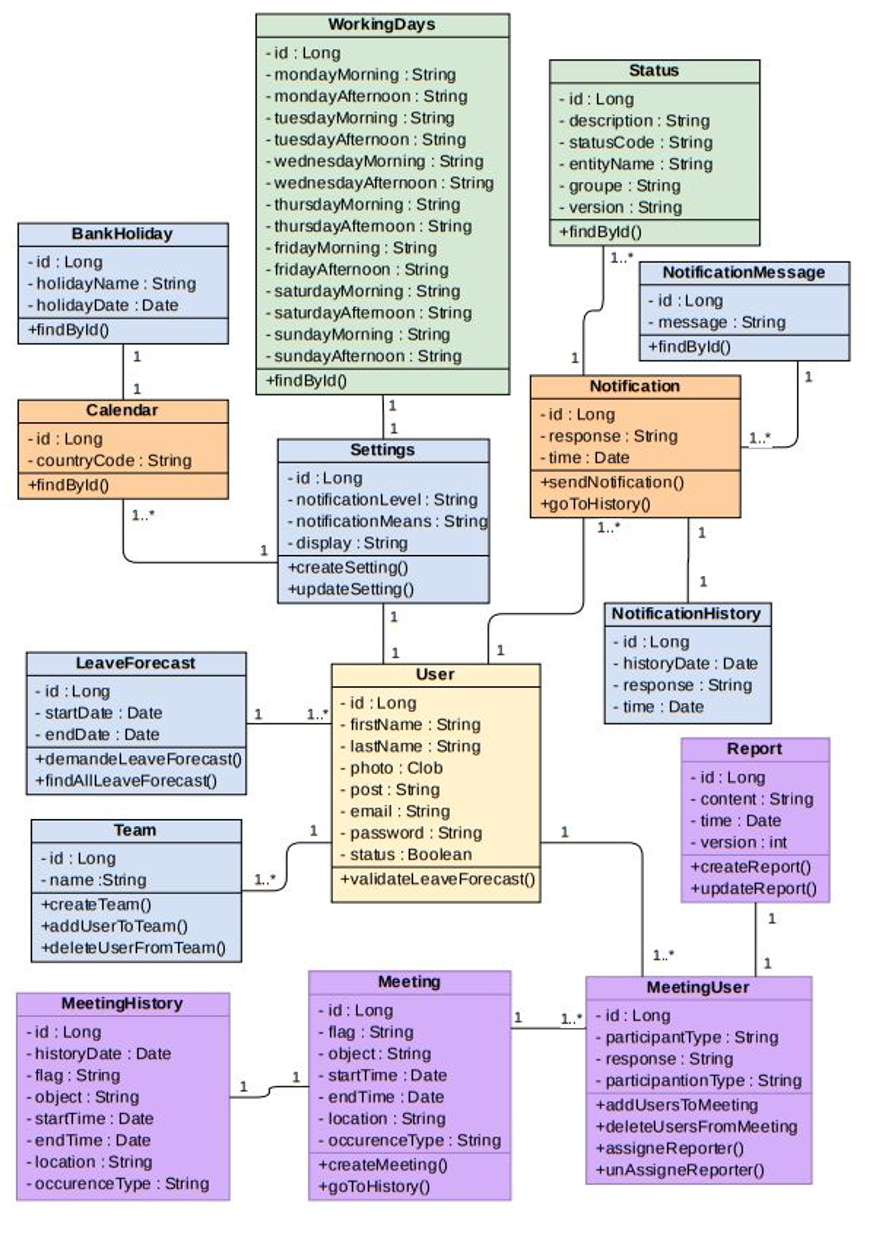
\includegraphics[scale=0.83]{figures/33anis2.png}
    \caption{Diagramme de classes «Gestion des Réunions, Notifications, Équipe et Paramétrage»}
    \label{fig:class_P2}
\end{figure}\newpage
\subsubsection{Diagramme de classes « Gestion de Projet »}
\hspace{4mm}Le diagramme de classes de la figure \ref{fig:class_P3} illustre toutes les entités indispensables à la gestion de projet. 
\begin{figure}[h]
    \centering
    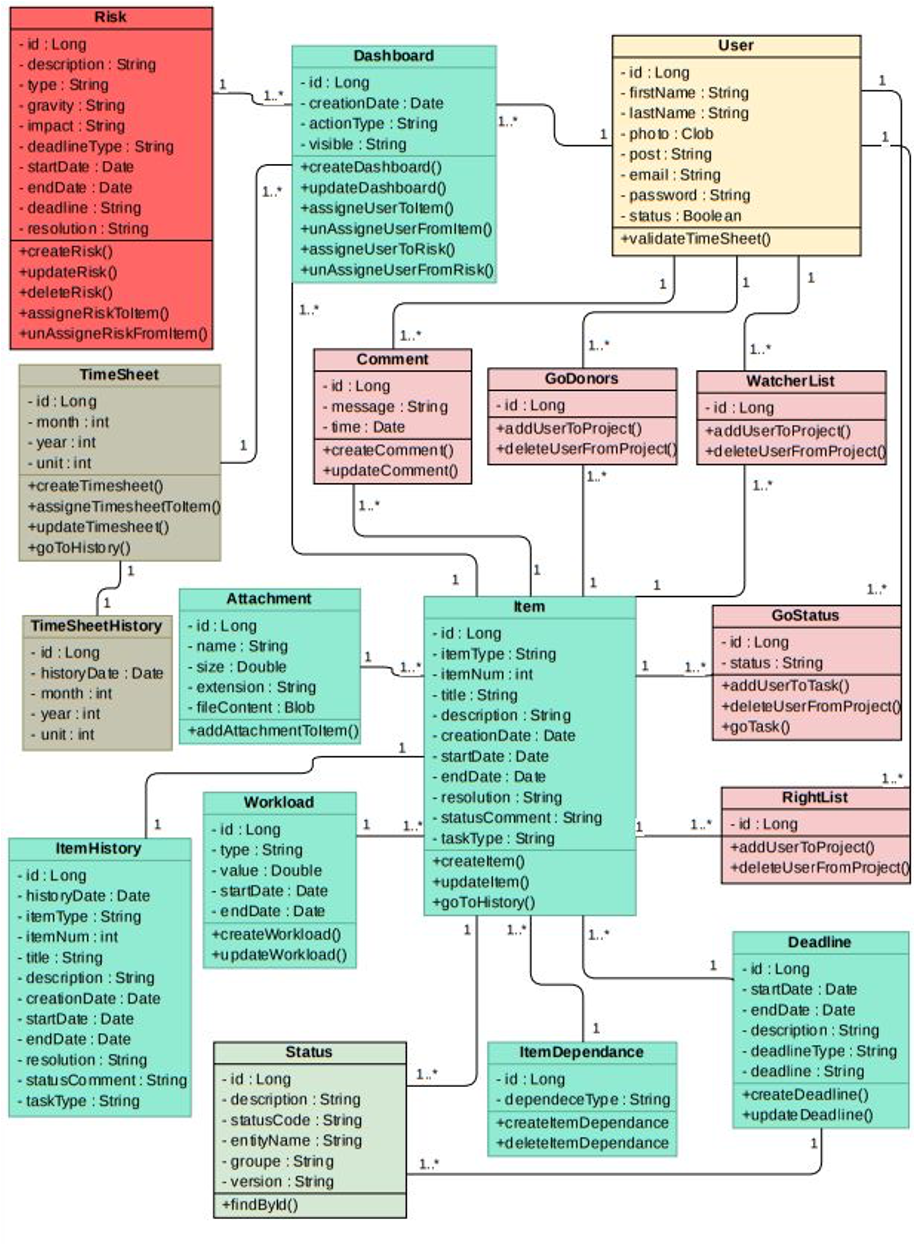
\includegraphics[scale=0.84]{figures/33anis3.png}
    \caption{Diagramme de classes « Gestion de Projet »}
    \label{fig:class_P3}
\end{figure}\newpage
\subsection{	Diagrammes de séquence }
\hspace{4mm}Le diagramme de séquence est une représentation séquentielle du déroulement des traitements et des interactions entre les éléments du système et/ou de ses acteurs \cite{14}. Avant d'entrer au menu du projet et faire l'ensemble des autres scénarios l'utilisateur doit se connecter. Le diagramme qui suit présente l'enchainement de la phase d'authentification. 
\newpage\par \textbf{	Authentification }
\begin{figure}[h]
    \centering
    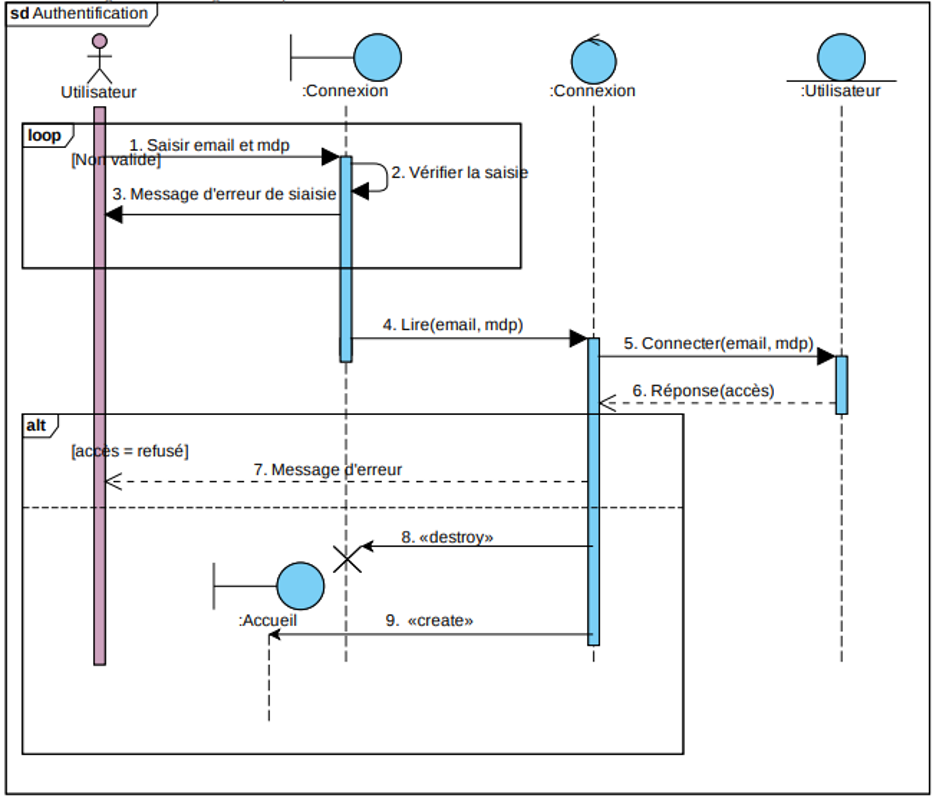
\includegraphics{figures/3anis5.png}
    \caption{Diagramme de Séquence " authentification "}
    \label{fig:Séquence_authentification}
\end{figure}
\par Description : 
\begin{itemize}
    \item L’utilisateur saisit son login et mot de passe pour accéder au système. Si les données introduites sont erronées, la page d’authentification se relance, sinon la page d’accueil du système s’ouvre.
\end{itemize}
\newpage\par \textbf{	Souscription  }
\begin{figure}[h]
    \centering
    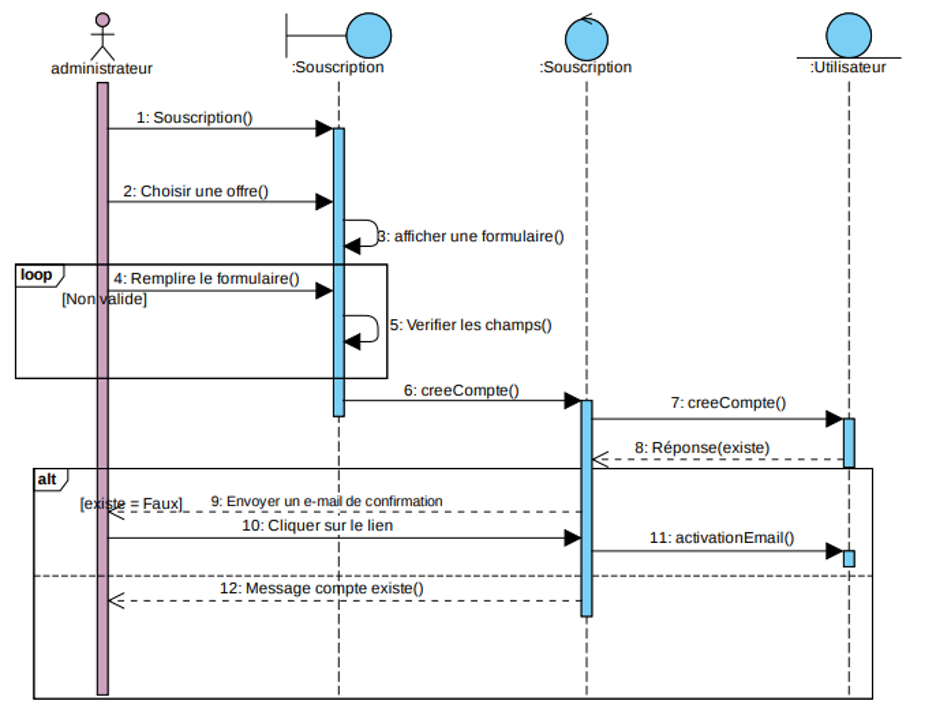
\includegraphics{figures/3anis6.png}
    \caption{Diagramme de Séquence " souscription "}
    \label{fig:Séquence_souscription}
\end{figure}
\par Description : 
\begin{itemize}
    \item L’utilisateur demande la souscription : une page s’affiche pour choisir une offre, selon l’offre choisie un formulaire à remplir s'affiche. Le système fait une vérification sur les champs, si tout est correct il envoie une requête d’inscription sinon un message d’erreur s’affiche sur les champs incorrects. Puis, selon les données saisies l'existence de ce compte est vérifié, si l’email existe un message d’erreur s’affiche, sinon les données seront enregistrées. 
\end{itemize}
\newpage\par \textbf{	Organiser une réunion   }
\begin{figure}[h]
    \centering
    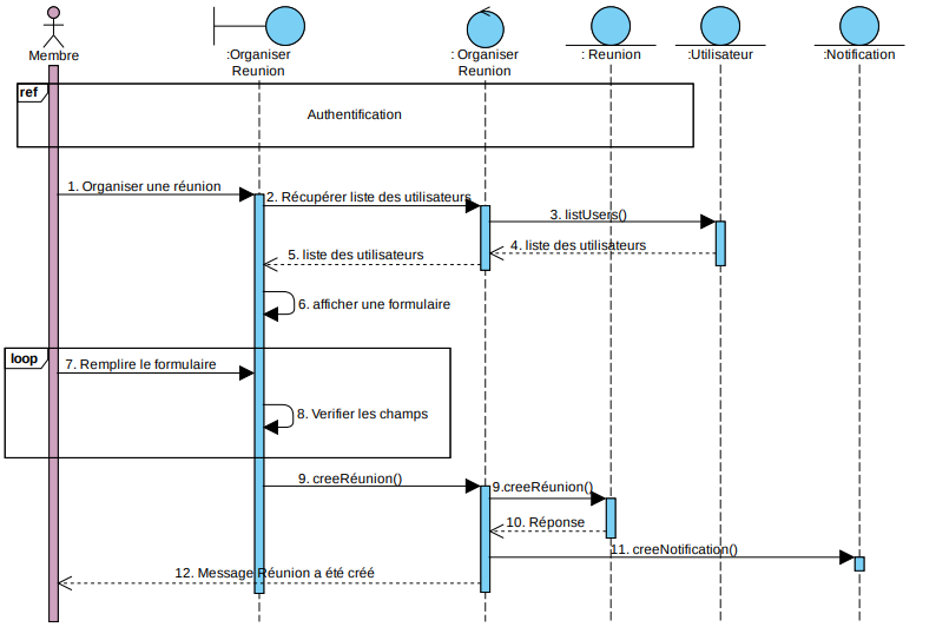
\includegraphics{figures/3anis7.png}
    \caption{Diagramme de Séquence "organiser une réunion"}
    \label{fig:Séquence_organiser}
\end{figure}
\par Description : 
\begin{itemize}
    \item 	L’utilisateur doit être authentifié pour organiser une réunion : un formulaire à remplir s'affiche. Il contient une liste des utilisateurs récupérée pour choisir les participants à la réunion. Le système fait une vérification sur les champs, si tout est correct il envoie une requête de création de réunion sinon un message d’erreur s’affiche sur les champs incorrects. Enfin, la réunion va être créée et selon les données saisies une notification sera envoyée à tous les participants.  
\end{itemize}
\section*{	Conclusion}
\hspace{4mm} 
Dans ce chapitre, nous avons présenté la conception de notre système. Nous avons détaillé l’architecture logiciel et nous avons établi le diagramme de classes et quelques diagrammes de séquences. Dans le dernier chapitre nous passerons à la phase de réalisation de tout ce qui a été défini et conçu tout au long des parties précédentes.




\chapter{Réalisation } \label{ch:réalis}
\hspace{4mm}Afin de finaliser notre projet la partie réalisation est d'autant plus importante que la phase de conception. Dans ce chapitre nous allons tout d'abord décrire les outils de développement adoptés pour la réalisation de notre application. Ensuite nous présenterons quelques interfaces de l'application.
\section{	Environnement de travail}
\subsection{	Environnement logiciel }
\subsubsection{	Outils logiciels}
\begin{itemize}
    \item 	Spring Tool Suite 
\end{itemize}
\par Spring Tool Suite est un IDE pour développer des applications Spring. Il s'agit d'un environnement de développement basé sur Eclipse. Il fournit un environnement prêt à l'emploi pour implémenter, exécuter, déployer et déboguer l'application. Il valide notre application et fournit des correctifs rapides pour les applications. \cite{5}
\newline
\begin{figure}[h]
    \centering
    
\includegraphics[scale=0.5]{figures/3333anis5.png}
    \caption*{}
    \label{fig:logo_STS}
\end{figure}\newpage
\begin{itemize}
    \item 	Visual Studio
\end{itemize}
\par Visual Studio Code est un éditeur du code léger et puissant supportant le travail avec TypeScript et Angular. Il dispose d’un éco système riche d’extensions qui nous a énormément aidés au cours du développement de notre application Web \cite{6}.
\begin{figure}[h]
    \centering
    
\includegraphics{figures/33anis6.png}
    \caption*{}
    \label{fig:logo_VS}
\end{figure}
\begin{itemize}
    \item 	Postman 
\end{itemize}
\par C’est une plateforme de collaboration qui se focalise sur les tests des APIs. Nous l’avons utilisé pour tester nos propres APIs \cite{7}.
\begin{figure}[h]
    \centering
    
\includegraphics{figures/33anis7.png}
    \caption*{}
    \label{fig:logo_POSTMAN}
\end{figure}
\begin{itemize}
    \item 	Gitlab 
\end{itemize}
\par GitLab est la première et unique application pour le développement, la sécurité et l’exploitation de logiciels, prenant en charge les DevOps simultanés. Elle permet d’accélérer ainsi le cycle de vie du logiciel et augmenter la vitesse de l’entreprise \cite{8}.
\begin{figure}[h]
    \centering
    
\includegraphics[scale=0.08]{figures/3333anis6.png}
    \caption*{}
    \label{fig:logo_GITLAB}
\end{figure}\newpage
\subsubsection{	Technologies}
\begin{itemize}
    \item 	Angular 
\end{itemize}
\par Il s’agit d’un framework développé et maintenu par Google. Il est basé sur le langage TypeScript et optimisé pour les applications Web composées d’une seule page côté client. Il est utilisé pour développer une interface client mono-page extrêmement robuste et adaptable \cite{9}.
\begin{figure}[h]
    \centering
    
\includegraphics{figures/33anis9.png}
    \caption*{}
    \label{fig:logo_ANGULAR}
\end{figure}
\begin{itemize}
    \item	Spring Boot 
\end{itemize}
\par Spring Boot est un framework open source, basé sur Java et utilisé dans la création de microservices. Il a été développé par Pivotal Team pour créer des applications Spring indépendantes et prêtes pour la production \cite{5}. 
\begin{figure}[h]
    \centering
    
\includegraphics{figures/33anis10.png}
    \caption*{}
    \label{fig:logo_SPRINGB}
\end{figure}
\begin{itemize}
    \item	Spring Security
\end{itemize}
\par Spring Security est un framework qui fournit l’authentification et d’autres fonctionnalités de sécurité pour les applications Java \cite{5}.
\begin{figure}[h]
    \centering
    
\includegraphics{figures/33anis11.png}
    \caption*{}
    \label{fig:logo_SPRINGS}
\end{figure}
\begin{itemize}
    \item	TypeScript
\end{itemize}
\par TypeScript est un langage de programmation libre et open source développé par Microsoft qui a pour but d'améliorer et de sécuriser la production de code JavaScript. \cite{10}
\begin{figure}[h]
    \centering
    
\includegraphics{figures/33anis13.png}
    \caption*{}
    \label{fig:logo_TYPES}
\end{figure}
\begin{itemize}
    \item	PostgreSQL
\end{itemize}
\par Est un puissant système de base de données relationnelle objet open source avec plus de 30 ans de développement actif qui lui a valu une solide réputation de fiabilité, de robustesse des fonctionnalités et de performances. \cite{11}
\begin{figure}[h]
    \centering
    
\includegraphics{figures/33anis14.png}
    \caption*{}
    \label{fig:logo_POSTGRE}
\end{figure}
\subsection{	Environnement matériel}
\begin{itemize}
    \item 	Ordinateurs portables
    \begin{itemize}
        \item DELL LATITUDE | E5510 ayant les caractéristiques suivantes :
        \begin{itemize}
            \item	Processeur Intel® Core™ i5 CPU M560 @ 2.67GHz, 2.67 GHz.
            \item 	Mémoire installée : 8Go, Disque dur SSD: 300 Go.
            \item	Système d’exploitation : Windows 10, 64 bits.
        \end{itemize}
    \end{itemize}
\end{itemize}\newpage
\section{	Interface de l'application}
\hspace{4mm}Cette partie détaillera la solution finale obtenue. Ainsi, nous présentons notre application à travers des imprimés écrans correspondants au travail réalisé.
\subsection{	Interfaces de souscription}
\hspace{4mm}Cette interface permet à l’utilisateur de choisir l’offre d’inscription.
\begin{figure}[h]
    \centering
    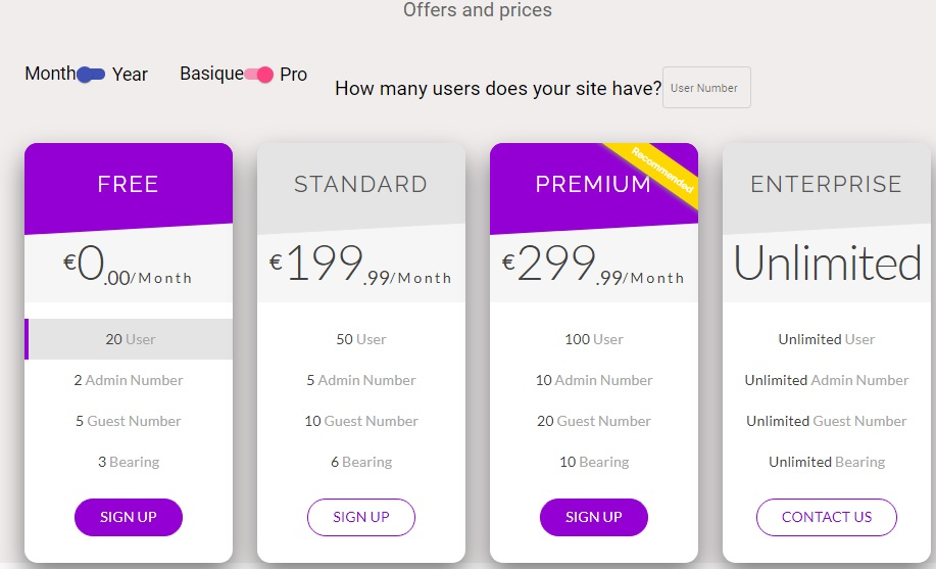
\includegraphics{figures/33anis15.png}
    \caption{Interface de sélection de l’offre d’inscription}
    \label{fig:interface_offre}
\end{figure}
\par La figure suivante présente l’interface d’inscription. L’utilisateur doit saisir son e-mail pour recevoir un mail d’activation. Une fois qu’on clique sur le lien reçu sur l’e-mail, le compte va être activé.\newpage
\begin{figure}[h]
    \centering
    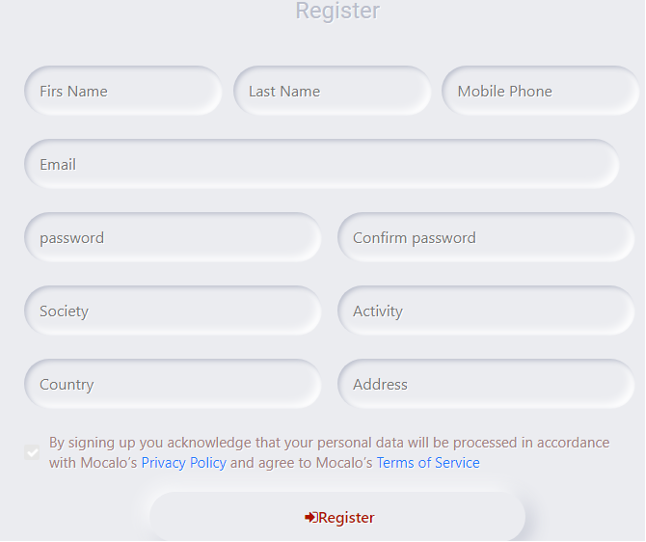
\includegraphics{figures/33anis16.png}
    \caption{Interface d’inscription}
    \label{fig:interface_inscri}
\end{figure}
\subsection{	Interface d’authentification}
\hspace{4mm}La figure \ref{fig:interface_auth} ci-dessous illustre l’interface d’accès à l’application. Elle implémente la fonction qui consiste à vérifier l’identité de l’utilisateur par un login et un mot de passe, afin de lui autoriser l’accès à cette application et lui offrir les services dédiés à son profil.
\begin{figure}[h]
    \centering
    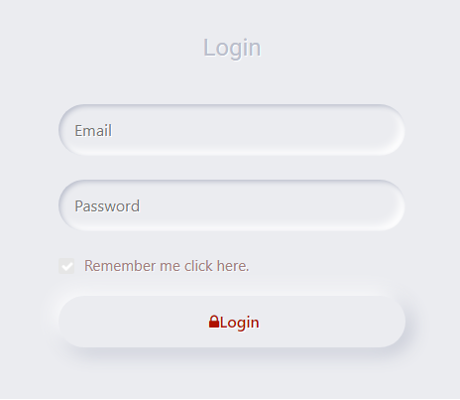
\includegraphics{figures/33anis17.png}
    \caption{Interface d’authentification}
    \label{fig:interface_auth}
\end{figure}
\subsection{	Interface de Dashboard}
\hspace{4mm}La figure ci-dessous \ref{fig:interface_dashb} présente l’interface de Dashboard, où l’utilisateur est en mesure de consulter les détails de tous les projets, les tâches et les anomalies. Il a  aussi la main pour gérer soit par ajout ou par modification  s’il a le droit. 
\newline
\begin{figure}[h]
    \centering
    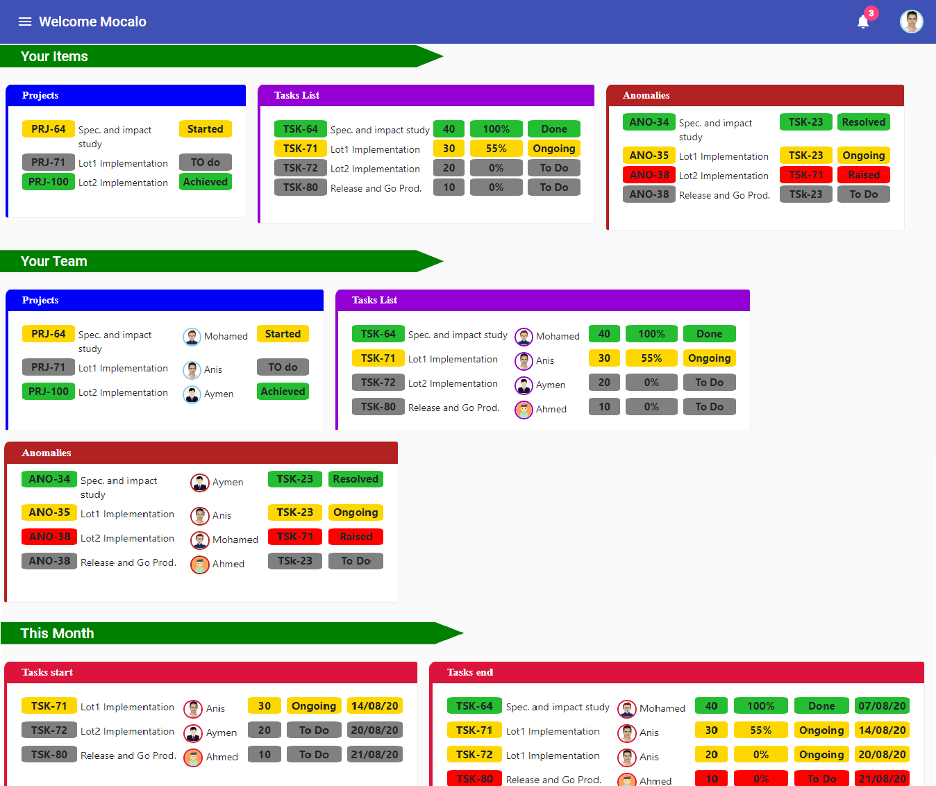
\includegraphics{figures/33anis18.png}
    \caption{Interface de Dashboard}
    \label{fig:interface_dashb}
\end{figure}\newpage
\subsection{	Interface d’une équipe}
\hspace{4mm}La figure ci-dessous \ref{fig:interface_équipe} présente l’interface d’une équipe sélectionnée, où l’utilisateur est en mesure de consulter les détails de tous les projets, les tâches et les anomalies pour une équipe sélectionnée. Cette interface offre aussi la possibilité de consulter la liste de ses membres.\newline
\begin{figure}[h]
    \centering
    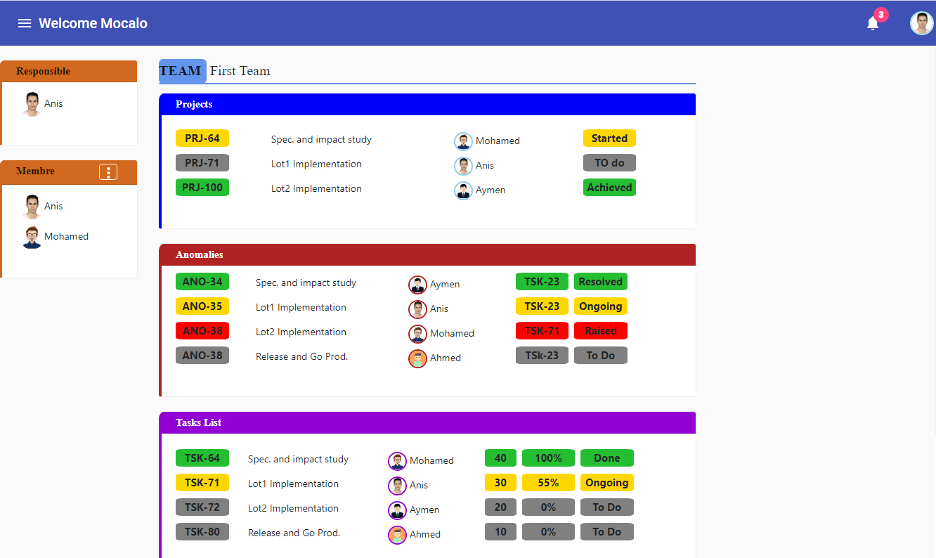
\includegraphics{figures/33anis19.png}
    \caption{Interface d’une équipe}
    \label{fig:interface_équipe}
\end{figure}\newpage
\subsection{	Interface d’un projet}
\hspace{4mm}La figure suivante présente les détails d’un projet. Cette interface offre aussi la possibilité de consulter la liste de ses titulaires de droits, la liste de ses observateurs, la liste de ses donneurs de go, la liste de ses tâches, les détails de ses planifications et les détails de ses risques.
\begin{figure}[h]
    \centering
    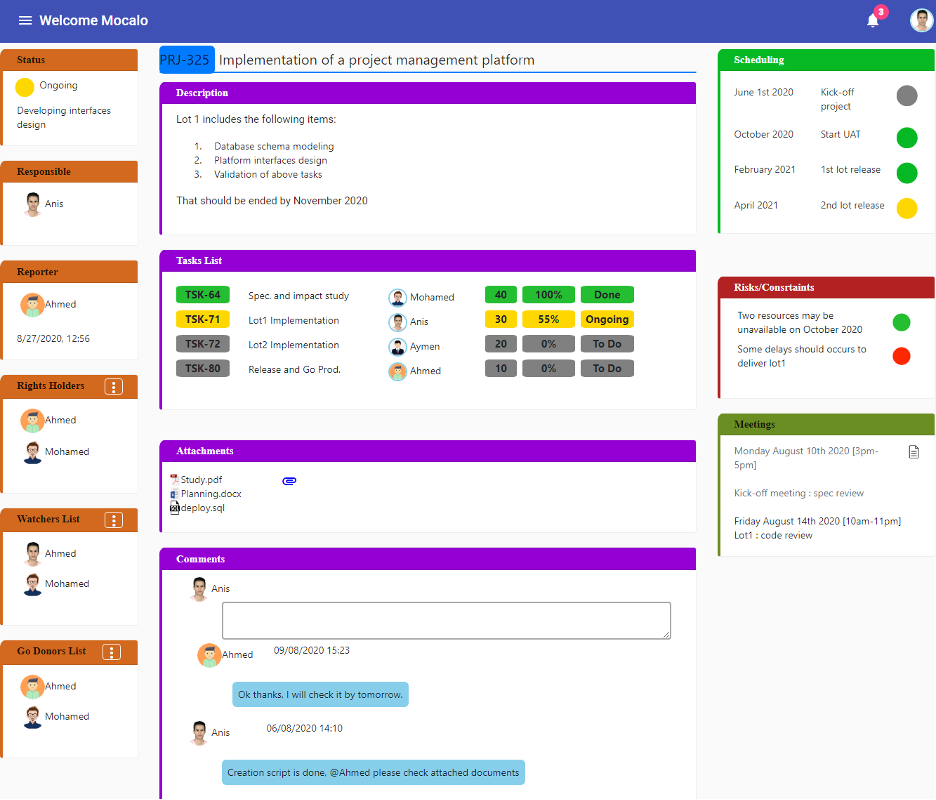
\includegraphics{figures/33anis20.png}
    \caption{Interface d’un projet}
    \label{fig:interface_projet}
\end{figure}\newpage
\subsubsection{	Interface de la liste des titulaires de droits }
\hspace{4mm}La figure suivante présente l’interface de la liste des titulaires de droits sur le projet.
\begin{figure}[h]
    \centering
    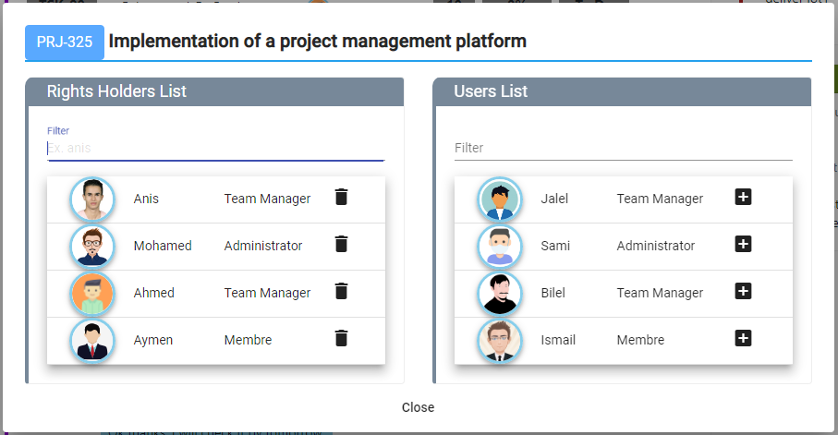
\includegraphics{figures/33anis21.png}
    \caption{Interface de la liste des titulaires de droits}
    \label{fig:interface_titulaires}
\end{figure}
\subsubsection{Interface de la liste des observateurs }
\hspace{4mm}La figure suivante présente l’interface de la liste des observateurs sur le projet.
\begin{figure}[h]
    \centering
    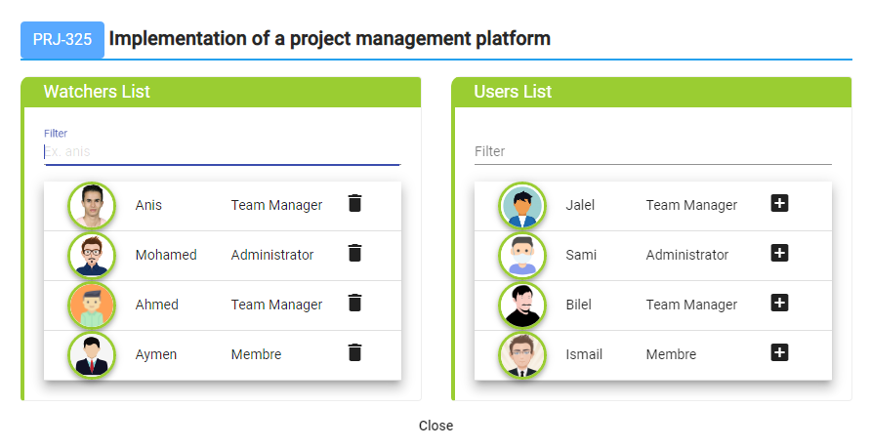
\includegraphics{figures/33anis22.png}
    \caption{Interface de la liste des observateurs}
    \label{fig:interface_observateur}
\end{figure}\newpage
\subsubsection{Interface de la liste des donneurs de go }
\hspace{4mm}La figure suivante présente l’interface de la liste des donneurs de go sur le projet.
\begin{figure}[h]
    \centering
    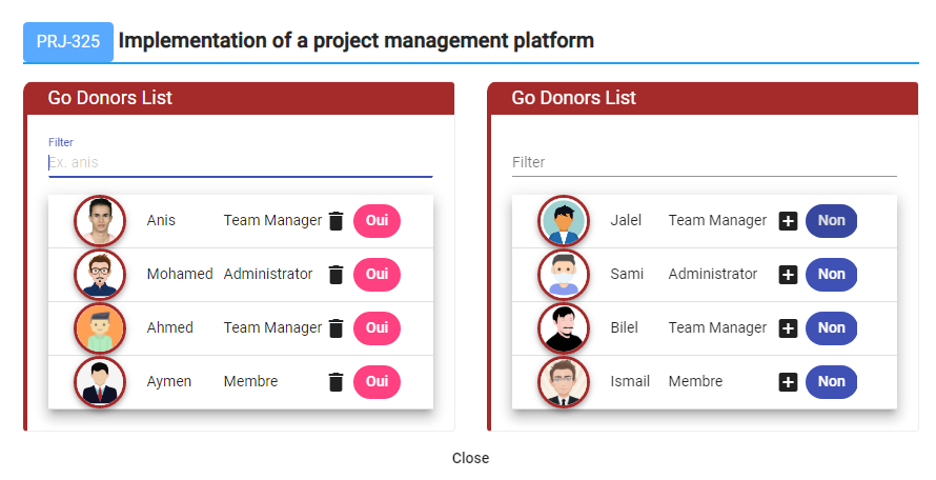
\includegraphics{figures/33anis23.png}
    \caption{Interface de la liste des donneurs de go}
    \label{fig:interface_donneur}
\end{figure}
\subsubsection{Interface de planification}
\hspace{4mm}La figure suivante présente les détails d’une planification.
\begin{figure}[h]
    \centering
    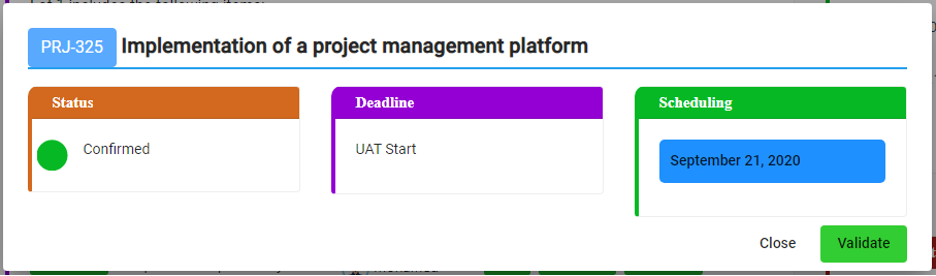
\includegraphics{figures/33anis24.png}
    \caption{Interface de planification de projet}
    \label{fig:interface_planification}
\end{figure}\newpage
\subsubsection{Interface d’un risque }
\hspace{4mm}La figure suivante présente les détails d’un risque.
\begin{figure}[h]
    \centering
    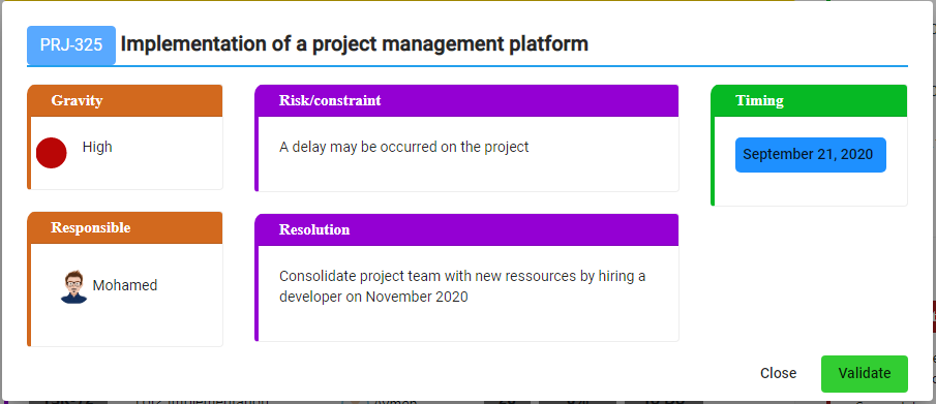
\includegraphics{figures/33anis25.png}
    \caption{Interface d’un risque}
    \label{fig:interface_risque}
\end{figure}\newpage
\subsection{Interface d’une tâche }
\hspace{4mm}La figure suivante présente les détails d’une tâche. Cette interface offre aussi la possibilité de consulter les détails d’une planification et les détails d’un risque.
\begin{figure}[h]
    \centering
    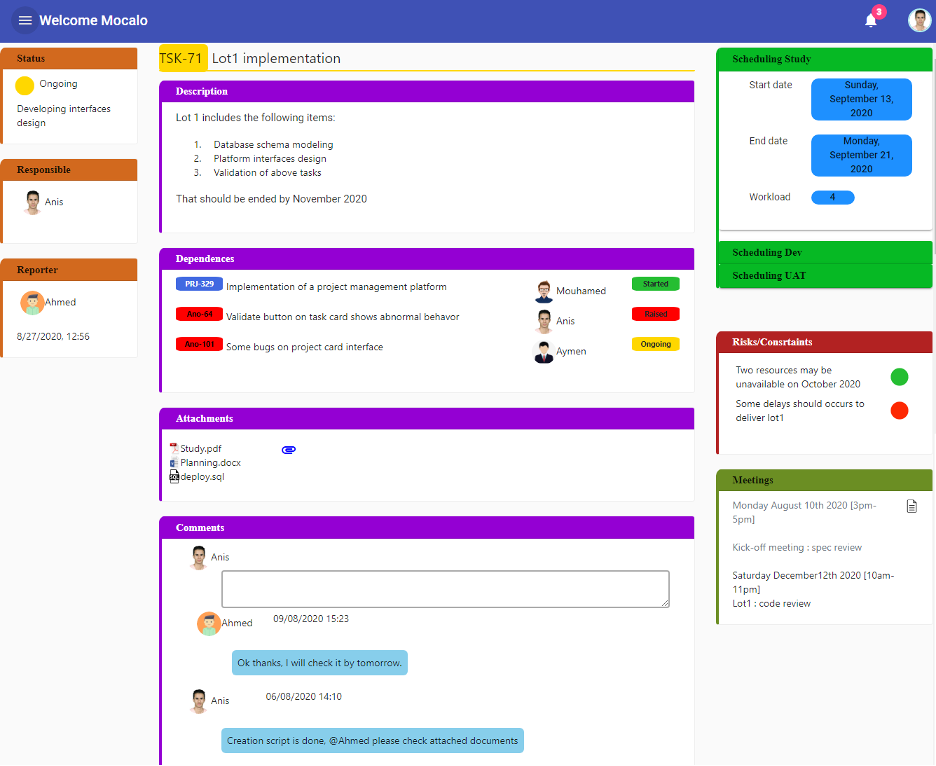
\includegraphics{figures/33anis26.png}
    \caption{Interface d’une tâche}
    \label{fig:interface_tache}
\end{figure}\newpage
\subsection{	Interface d'une anomalie }
\hspace{4mm}La figure suivante présente les détails d’une anomalie. Cette interface offre aussi la possibilité de consulter les détails d’une planification.
\begin{figure}[h]
    \centering
    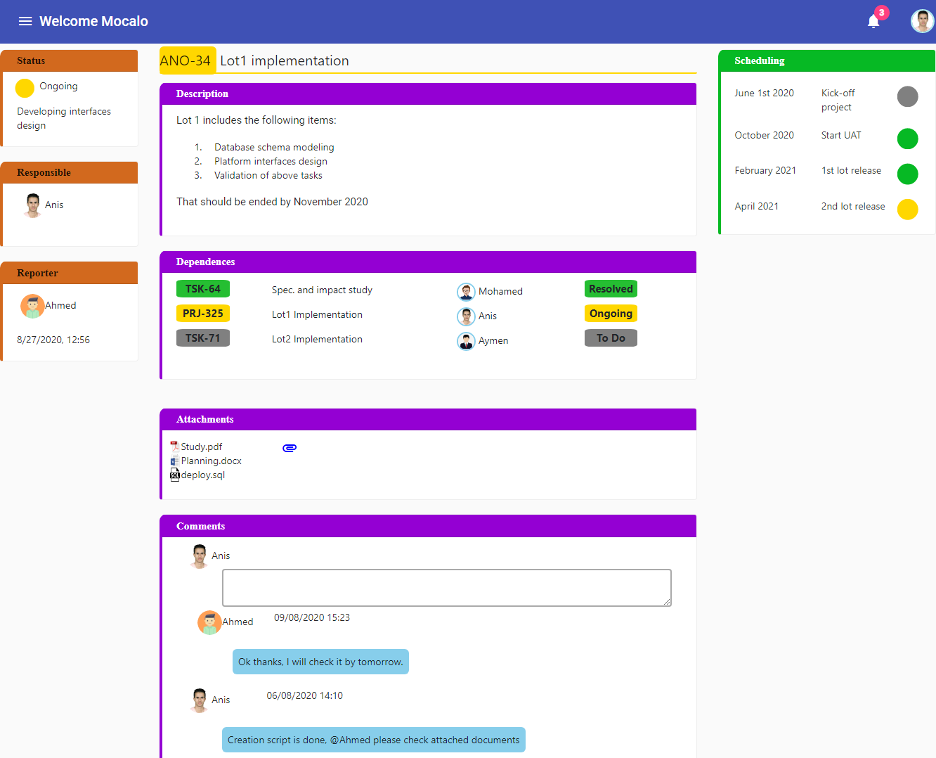
\includegraphics{figures/33anis27.png}
    \caption{Interface de l’anomalie}
    \label{fig:interface_anomalie}
\end{figure}\newpage
\subsection{	Interface d’une libération de tâche}
\hspace{4mm}La figure suivante présente les détails d’une libération de tâche. Cette interface offre aussi la possibilité de consulter les détails d’une planification.
\begin{figure}[h]
    \centering
    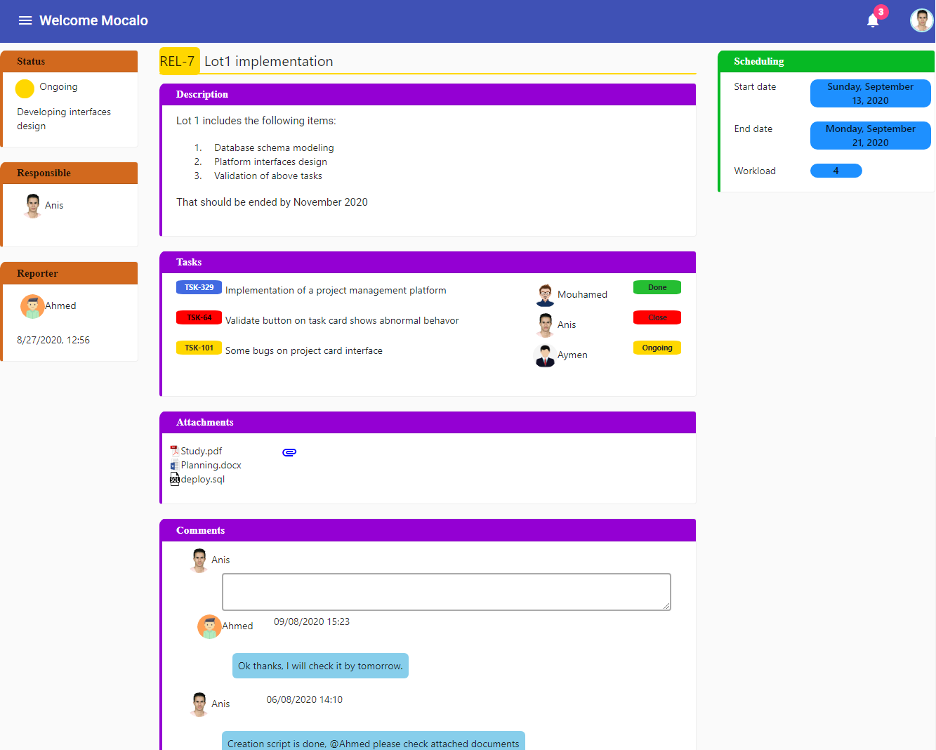
\includegraphics{figures/33anis28.png}
    \caption{Interface d’une libération}
    \label{fig:interface_liberation}
\end{figure}\newpage
\subsection{	Interface d'un emploi du temps  }
\hspace{4mm}La figure suivante présente l’interface d'un emploi du temps.
\begin{figure}[h]
    \centering
    \includegraphics[scale=0.5]{figures/3333anis7.png}
    \caption{Interface d'un emploi du temps}
    \label{fig:interface_timesheet}
\end{figure}
\subsection{Interface de prévision de congé}
\hspace{4mm}La figure suivante présente l’interface de la liste de prévision de congé.
\begin{figure}[h]
    \centering
    \includegraphics[scale=0.65]{figures/a5.png}
    \caption{Interface de prévision de congé}
    \label{fig:interface_congé}
\end{figure}\newpage
\subsection{	Interfaces de réunion}
\hspace{4mm}Cette interface permet à l’utilisateur de fixer une date de réunion. \newline
\begin{figure}[h]
    \centering
    \includegraphics[scale=0.35]{figures/a6.png}
    \caption{Interface de sélection d'une date de  réunion}
    \label{fig:interface_reunion}
\end{figure}\newline
\hspace{4mm}La figure suivante présente l’interface de création d'une réunion.  \newline
\begin{figure}[h]
    \centering
    \includegraphics[scale=0.35]{figures/a7.png}
    \caption{Interface de création d'une réunion}
    \label{fig:interface_creation_reunion}
\end{figure}\newpage
\par La figure suivante présente l’interface résultat de la création d'une réunion.
\begin{figure}[h]
    \centering
    \includegraphics[scale=0.35]{figures/a8.png}
    \caption{Interface résultat de la création d'une réunion}
    \label{fig:interface_resultcreation_reunion}
\end{figure}
\subsection{	Interface de Notification }
\hspace{4mm}La figure suivante présente l’interface de Notification.
\begin{figure}[h]
    \centering
    \includegraphics{figures/33anis3'.png}
    \caption{Interface de Notification}
    \label{fig:interface_notification}
\end{figure}
\section*{	Conclusion}
\hspace{4mm} 
Dans ce dernier chapitre, nous avons décrit l'environnement du travail et présenté les principales interfaces de l'application réalisée.

\addcontentsline{toc}{chapter}{Conclusion Générale}
\chapter*{ Conclusion Générale}
\markboth{}{}
\mark{ COONCLUSION GÉNÉRALE}
\hspace{4mm}Ce projet avait pour but la conception et le développement d’une plateforme de gestion de projet. Cette plateforme permet de créer un environnement de travail de transparence, d’engagement et de responsabilité, pour optimiser le travail d’équipe. 

\hspace{4mm}

Durant la période de réalisation du projet, nous avons dégagé les besoins fonctionnels du client afin de parvenir à la conception de notre solution. Ensuite, nous avons installé les outils de travail nécessaires. Pour entamer finalement la phase de réalisation de l'application.

\hspace{4mm}

Cette formidable expérience m'a permis de maîtriser des nouveaux langages de développement, tels que SpringBoot
pour le développement back-end et Angular pour le développement front-end. Elle m'a permis également d'intégrer et de voir de près le milieu professionnel, ce qui m'a appris des compétences techniques et pratiques consolidant mes acquis théoriques pendant mes années d'études. Pendant ce stage, j'ai admis un certain nombre de qualités permettant d'intégrer le marché d’emploi en en nouant un lien entre la formation théorique et la réalité professionnelle. En effectuant ce stage, j'ai acquis certaines attitudes que je n'avais pas avant, à savoir : 

\par La confiance en soi, le respect de l'horaire de travail, le respect du métier, le respect des supérieurs et collègues et la rapidité d’exécution des tâches. 

\par
A la fin, j’espère que ce modeste travail apportera la satisfaction des membres de Jury et de toute l’équipe de MOCALO SERVICES. 

\addcontentsline{toc}{chapter}{Webographie} 
\renewcommand\bibname{Webographie}
\begin{thebibliography}{20}
\bibitem{1} \url{ http://prive.iutenligne.net/iuRxM0CThIXDIjzG/informatique/langages/kettaf/UML/04modeleconceptuel/0302acteurs.html} (Consulté le 15/06/2020).
\bibitem{2} \url{ http://orm.bdpedia.fr/mvc.html} (Consulté le 20/07/2020).
\bibitem{3} \url{ https://bezkoder.com/spring-boot-jwt-mysql-spring-security-architecture/} (Consulté le 05/10/2020).
\bibitem{4} \url{  https://bezkoder.com/angular-jwt-authentication/} (Consulté le 06/10/2020).

\bibitem{5} \url{  https://spring.io/} (Consulté le 15/09/2020).
\bibitem{6} \url{ https://code.visualstudio.com} (Consulté le 04/08/2020).
\bibitem{7} \url{  https://www.postman.com/} (Consulté le 09/10/2020).
\bibitem{8} \url{https://about.gitlab.com/} (Consulté le 23/07/2020).
\bibitem{9} \url{ https://angular.io/} (Consulté le 17/08/2020).
\bibitem{10} \url{  https://www.typescriptlang.org/} (Consulté le 17/08/2020).
\bibitem{11} \url{  https://www.postgresql.org/} (Consulté le 17/08/2020).
\bibitem{12} \url{https://web.maths.unsw.edu.au/~lafaye/CCM/initiation/client.htm} (Consulté le 21/07/2020).
\bibitem{13} \url{https://bezkoder.com/react-spring-boot-crud/} (Consulté le 06/10/2020).
\bibitem{14} \url{https://manurenaux.wp.imt.fr/2014/05/16/les-missions-dun-expert-uml/} (Consulté le 12/10/2020).
\end{thebibliography}

\printbibliography



\end{document}          
